% Template for PLoS
% Version 3.5 March 2018
%
% % % % % % % % % % % % % % % % % % % % % %
%
% -- IMPORTANT NOTE
%
% This template contains comments intended 
% to minimize problems and delays during our production 
% process. Please follow the template instructions
% whenever possible.
%
% % % % % % % % % % % % % % % % % % % % % % % 
%
% Once your paper is accepted for publication, 
% PLEASE REMOVE ALL TRACKED CHANGES in this file 
% and leave only the final text of your manuscript. 
% PLOS recommends the use of latexdiff to track changes during review, as this will help to maintain a clean tex file.
% Visit https://www.ctan.org/pkg/latexdiff?lang=en for info or contact us at latex@plos.org.
%
%
% There are no restrictions on package use within the LaTeX files except that 
% no packages listed in the template may be deleted.
%
% Please do not include colors or graphics in the text.
%
% The manuscript LaTeX source should be contained within a single file (do not use \input, \externaldocument, or similar commands).
%
% % % % % % % % % % % % % % % % % % % % % % %
%
% -- FIGURES AND TABLES
%
% Please include tables/figure captions directly after the paragraph where they are first cited in the text.
%
% DO NOT INCLUDE GRAPHICS IN YOUR MANUSCRIPT
% - Figures should be uploaded separately from your manuscript file. 
% - Figures generated using LaTeX should be extracted and removed from the PDF before submission. 
% - Figures containing multiple panels/subfigures must be combined into one image file before submission.
% For figure citations, please use "Fig" instead of "Figure".
% See http://journals.plos.org/plosone/s/figures for PLOS figure guidelines.
%
% Tables should be cell-based and may not contain:
% - spacing/line breaks within cells to alter layout or alignment
% - do not nest tabular environments (no tabular environments within tabular environments)
% - no graphics or colored text (cell background color/shading OK)
% See http://journals.plos.org/plosone/s/tables for table guidelines.
%
% For tables that exceed the width of the text column, use the adjustwidth 2222 as illustrated in the example table in text below.
%
% % % % % % % % % % % % % % % % % % % % % % % %
%
% -- EQUATIONS, MATH SYMBOLS, SUBSCRIPTS, AND SUPERSCRIPTS


% IMPORTANT
% Below are a few tips to help format your equations and other special characters according to our specifications. For more tips to help reduce the possibility of formatting errors during conversion, please see our LaTeX guidelines at http://journals.plos.org/plosone/s/latex
%
% For inline equations, please be sure to include all portions of an equation in the math environment.  For example, x$^2$ is incorrect; this should be formatted as $x^2$ (or $\mathrm{x}^2$ if the romanized font is desired).
%
% Do not include text that is not math in the math environment. For example, CO2 should be written as CO\textsubscript{2} instead of CO$_2$.
%
% Please add line breaks to long display equations when possible in order to fit size of the column. 
%
% For inline equations, please do not include punctuation (commas, etc) within the math environment unless this is part of the equation.
%
% When adding superscript or subscripts outside of brackets/braces, please group using {}.  For example, change "[U(D,E,\gamma)]^2" to "{[U(D,E,\gamma)]}^2". 
%
% Do not use \cal for caligraphic font.  Instead, use \mathcal{}
%
% % % % % % % % % % % % % % % % % % % % % % % % 
%
% Please contact latex@plos.org with any questions.
%
% % % % % % % % % % % % % % % % % % % % % % % %

\documentclass[10pt,letterpaper]{article}
%\usepackage[top=0.85in,left=2.75in,footskip=0.75in]{geometry}
\usepackage{fullpage}

% amsmath and amssymb packages, useful for mathematical formulas and symbols
\usepackage{amsmath,amssymb}
\usepackage{latexsym}
\usepackage{color}
\usepackage{graphics}
\usepackage{xspace}
\usepackage{graphicx}  %Required
\usepackage{epsfig}
\usepackage{amsthm}
\usepackage{pdfpages}
\usepackage{algorithm}
\usepackage[noend]{algorithmic}
%\usepackage[noend]{algpseudocode}

% Use adjustwidth environment to exceed column width (see example table in text)
\usepackage{changepage}

% Use Unicode characters when possible
\usepackage[utf8x]{inputenc}

% textcomp package and marvosym package for additional characters
\usepackage{textcomp,marvosym}

% cite package, to clean up citations in the main text. Do not remove.
\usepackage{cite}

% Use nameref to cite supporting information files (see Supporting Information section for more info)
\usepackage{nameref,hyperref}

% line numbers
\usepackage[right]{lineno}

% ligatures disabled
\usepackage{microtype}
\DisableLigatures[f]{encoding = *, family = * }

% color can be used to apply background shading to table cells only
\usepackage[table]{xcolor}

% array package and thick rules for tables
\usepackage{array}

% create "+" rule type for thick vertical lines
\newcolumntype{+}{!{\vrule width 2pt}}

% create \thickcline for thick horizontal lines of variable length
\newlength\savedwidth
\newcommand\thickcline[1]{%
  \noalign{\global\savedwidth\arrayrulewidth\global\arrayrulewidth 2pt}%
  \cline{#1}%
  \noalign{\vskip\arrayrulewidth}%
  \noalign{\global\arrayrulewidth\savedwidth}%
}

\newcommand{\hide}[1]{}

% \thickhline command for thick horizontal lines that span the table
\newcommand\thickhline{\noalign{\global\savedwidth\arrayrulewidth\global\arrayrulewidth 2pt}%
\hline
\noalign{\global\arrayrulewidth\savedwidth}}


% Remove comment for double spacing
%\usepackage{setspace} 
%\doublespacing

\newcommand{\alg}{\textsc{HaiDetect}\xspace}
\newcommand{\algt}{\textsc{HaiEarlyDetect}\xspace}
\newcommand{\celf}{\textsc{Celf}\xspace}

% Text layout
\raggedright
\setlength{\parindent}{0.5cm}
\textwidth 5.25in 
\textheight 8.75in

% Bold the 'Figure #' in the caption and separate it from the title/caption with a period
% Captions will be left justified
\usepackage[aboveskip=1pt,labelfont=bf,labelsep=period,justification=raggedright,singlelinecheck=off]{caption}
\renewcommand{\figurename}{Fig}

% Use the PLoS provided BiBTeX style
%%%%%%%%%%change this for the final submission %%%%%%%%%%%%%
%\bibliographystyle{plos2015}

% Remove brackets from numbering in List of References
\makeatletter
\renewcommand{\@biblabel}[1]{\quad#1.}
\makeatother



% Header and Footer with logo
\usepackage{lastpage,fancyhdr,graphicx}
\usepackage{epstopdf}
%\pagestyle{myheadings}
\pagestyle{fancy}
\fancyhf{}
%\setlength{\headheight}{27.023pt}
%\lhead{\includegraphics[width=2.0in]{PLOS-submission.eps}}
\rfoot{\thepage/\pageref{LastPage}}
\renewcommand{\headrulewidth}{0pt}
\renewcommand{\footrule}{\hrule height 2pt \vspace{2mm}}
\fancyheadoffset[L]{2.25in}
\fancyfootoffset[L]{2.25in}
\lfoot{\today}

%% Include all macros below



\DeclareMathOperator*{\argmax}{arg\,max}
\DeclareMathOperator*{\argmin}{arg\,min}


\newtheorem{problem}{Problem}
\newtheorem{lemma}{Lemma}
\newtheorem{defn}{Definition}


\newcommand{\Ss}{\mathcal{S}}
\newcommand{\R}{\mathcal{R}}
\newcommand{\cc}{\mathcal{C}}
\newcommand{\I}{\mathcal{I}}
\newcommand{\vr}{\mathbf{r}}
\newcommand{\vc}{\mathbf{c}}
\newcommand{\va}{\mathbf{a}}
\newcommand{\ve}{\mathbf{e}}
\newcommand{\vb}{\mathbf{b}}
\newcommand{\x}{\mathbf{x}}
\newcommand{\y}{\mathbf{y}}
\newcommand{\curV}{\hat{\vr}}
\newcommand{\optV}{\vr^*}

\newcommand{\forBryan}[1]{{\color{red} #1}}
\newcommand{\forAnil}[1]{{\color{blue} #1}}
\newcommand{\forJose}[1]{{\color{teal} #1}}
\newcommand{\frombijaya}[1]{{\color{blue} #1}}
\newcommand{\fromBryan}[1]{{{\bf \textcolor{blue}{bryan says:}}
\textcolor{green}{#1}}}
\newcommand{\frombryan}[1]{{{\bf Bryan says:} #1}}
\newcommand{\fromanil}[1]{{{\bf \textcolor{red}{anil says:}} \textcolor{red}{#1}}}
\newcommand{\addedbyanil}[1]{{{\bf \textcolor{red}{added by anil:}} \textcolor{red}{#1}}}
\newcommand{\reminder}[1]{{\bf *** #1 *** }}

%% END MACROS SECTION

%\newcommand{\hide}[1]{}



%%%%%%%%%%%%%%%%%%%%%
\iffalse
\documentclass[11pt]{amsart}

\usepackage{graphicx}
\usepackage{caption}
%\usepackage{subcaption}
\usepackage{url}

\usepackage{algorithm}
\usepackage[noend]{algorithmic}
\usepackage{amsmath,amsfonts,amssymb}
%%\usepackage{fullpage} %[cm]
\usepackage{lmodern} % enhanced version of computer modern
\usepackage[T1]{fontenc} % for hyphenated characters
%%\usepackage{amsmath}
%%\usepackage{amssymb}
\usepackage{microtype}
\usepackage{enumerate}
\usepackage{ctable} % provides toprule, bottomrule, midrule
%\usepackage[ruled,linesnumbered]{algorithm2e}
\usepackage{amsthm}
\usepackage{graphicx}
\usepackage{subfig}
\DeclareCaptionType{copyrightbox}
\usepackage{color}
\def \tommy #1{{\color{red} #1}}
\newcommand{\expect}{\mathrm{Exp}}
\newcommand{\hide}[1]{}
\newtheorem{theorem}{Theorem} % {\bfseries}{\itshape}
\newtheorem{lemma}{Lemma}[section]{\bfseries}{\itshape}
\newtheorem{corollary}{Corollary}[section]{\bfseries}{\itshape}
%\newdef{claim}{Claim}
%
%\theoremstyle{definition}
%\newtheorem{definition}[lemma]{Definition} % {\bfseries}{\itshape}
%
%\theoremstyle{remark}
\newtheorem{claim}[lemma]{Claim} % {\bfseries}{\itshape}
%
\DeclareMathOperator*{\argmin}{arg\,min}
\newcommand{\opt}{\mathrm{OPT}}
\newcommand{\degr}{\mathrm{d}}
\newcommand{\Vol}{\mathrm{Vol}}
\newcommand{\wmax}{w_{\max}}
\newcommand{\eps}{\epsilon}
\newcommand{\ceil}[1]{\left\lceil #1 \right\rceil}
\newcommand{\comment}[1]{\textcolor{red}{#1}}
\newcommand{\A}{\mathcal{A}}
\newcommand{\D}{\mathcal{D}}
\newcommand{\B}{\mathcal{B}}
\renewcommand{\S}{\mathcal{S}}
\newcommand{\I}{\mathcal{I}}
\newcommand{\J}{\mathcal{J}}
\newcommand{\T}{\mathcal{T}}
\newcommand{\V}{\mathcal{V}}
\newcommand{\U}{\mathcal{U}}
\newcommand{\M}{\mathcal{M}}
\newcommand{\R}{\mathcal{R}}
\renewcommand{\P}{\mathcal{P}}
\newcommand{\e}{\mathcal{E}}
\newcommand{\cost}{\,\text{cost}\,}


\DeclareMathOperator*{\nodes}{nodes}
\DeclareMathOperator*{\walks}{walks}
\DeclareMathOperator*{\ct}{count}

\setlength{\oddsidemargin}{-0.1in}
\setlength{\evensidemargin}{-0.1in}
\setlength{\textheight}{9in}
\setlength{\textwidth}{6.5in}
\setlength{\topmargin}{-0.25in}
%\baselineskip=1.10\normalbaselineskip
\renewcommand{\baselinestretch}{1.05}

\numberwithin{equation}{section}


\title{Optimizing access to healthcare facilities during pandemic outbreaks}
%\author{}
\date{}
%
\begin{document}
\maketitle
%
%%%%%%%%%%%%%%
\fi

\newcommand{\OPT}{\text{OPT}}
\newcommand{\KMED}{\text{kmed}}
\newcommand{\CAPKMED}{\text{cap-kmed}}
\newcommand{\LP}{\text{LP}}
\newcommand{\F}{\mathcal{F}}
\newcommand{\C}{\mathcal{C}}
\newcommand{\objcenter}{\phi_{max}}
\newcommand{\objmedian}{\phi_{avg}}
\newcommand{\probstatic}{\textsc{FacilityPlanning}}
\newcommand{\probkernel}{\textsc{KernelFacility}}
\newcommand{\probinc}{\textsc{IncrementalFacility}}
\newcommand{\algokmedstatic}{\textsc{StaticKMed}}
\newcommand{\algokmedonline}{\textsc{OnlineKMed}}
\newcommand{\algokernelkmed}{\textsc{KernelKMed}}

\newcommand{\red}[1]{\textcolor{red}{#1}}

%\newtheorem{proposition}{Proposition}[section]{\bfseries}{\itshape}
\newtheorem{proposition}{Proposition}{\bfseries}{\itshape}
\newtheorem{theorem}{Theorem} % {\bfseries}{\itshape}
%%\newtheorem{lemma}{Lemma}[section]{\bfseries}{\itshape}
\newtheorem{corollary}{Corollary}{\bfseries}{\itshape}

\begin{document}

% Title must be 250 characters or less.
\begin{flushleft}
{\Large
\textbf\newline{Optimizing access to healthcare facilities during pandemic outbreaks}
}\newline
% Insert author names, affiliations and corresponding author email (do not include titles, positions, or degrees).

\end{flushleft}

\begin{abstract}
As the 2014 Ebola outbreak showed, providing timely access to healthcare resources,
e.g., diagnostic centers and hospitals, is crucial for controlling the spread of a
pandemic disease. However, this turns out to be a challenging multi-criteria
optimization problem. In this paper, we use rigorous methods from location theory
to study these problems. Specifically, we consider what
kinds of objectives are important, and how facilities should be deployed in order to
optimize those objectives, especially when they are being deployed incrementally.
Using simulated outbreak data for the 2014 Ebloa outbreak in West Africa,
we find that the specific objective, i.e., individual vs. social cost (e.g., travel time 
to the nearest open facility), has a significant impact,
and that the use of epidemic forecasts can greatly improve the quality of the solutions.
In the typical setting where the number of facilities to be deployed is not known ahead of time,
we also demonstrate a new approach for incrementally deploying facilities, which
leads to solutions with cost very close to the optimal solutions. In particular, we find
there are some \emph{kernel} locations, at which facilities can be deployed initially,
without affecting the quality of the solutions.
Thus, our results suggest a simple and efficient method for deploying healthcare resources
during pandemic outbreaks.

%Motivated by the Ebola outbreak and the challenges arising in the response to it,
%we study the problem of how to deploy healthcare facilities in the event of a
%an epidemic outbreak in a large region. Specifically, we consider the questions
%of what objectives are important, and how should facilities be deployed in order to
%optimize those objectives. Our main contributions
%are threefold. First, we find there is a significant difference between
%individual and social cost (e.g., travel time to the nearest open facility).
%Second, we find that using forecasts of epidemic incidence can greatly improve
%the effectiveness of facility location. Finally, there are core facilities,
%and deploying these initially, and deploying the subsequent ones based on
%the epidemic incidence leads to more effective solutions.
\end{abstract}

% Please keep the Author Summary between 150 and 200 words
% Use first person. PLOS ONE authors please skip this step. 
% Author Summary not valid for PLOS ONE submissions.   
\section*{Author summary}

summary


\linenumbers

\section*{Introduction}

\red{make text more current}

The 2014 Ebola outbreak was the largest in history, accounting for more than 11,300
deaths in West Africa. Starting in Guinea in December 2013 \cite{Baize2014}, 
the epidemic quickly spread to the neighboring countries,
and sustained autochthonous transmission was seen in Liberia and Sierra Leone
by March, 2014.  The health infrastructure in the West African countries of Guinea, Sierra Leone and Liberia
was severely strained by this outbreak. Patients had to travel long distances
by various modes of transport to reach a hospital, or worse, a holding center
before they could be transferred to a hospital,\footnote{%
\url{http://www.cdc.gov/mmwr/preview/mmwrhtml/mm6439a4.htm}}
which played a big role in increasing transmission in the initial stages of the outbreak.
As part of the response efforts,
Ebola Treatment Centers (ETCs) were set up with international help
in order to isolate and treat infected individuals.
However, this was done without necessarily
optimizing access to healthcare for infected patients, so some of the ETCs
were underutilized.  For instance, several
ETCs never saw any patients.\footnote{%
\url{http://www.nytimes.com/2015/04/12/world/africa/idle-ebola-clinics-in-liberia-are-seen-as-misstep-in-us-relief-effort.html?_r=0}}.
While there might be a multitude of reasons (which are still being studied by
the public health community), some of these include: limitations in forecasting
Ebola spread (including lack of data and behavioral adaptations at all levels), 
delays in response, and the disconnect between logistical planning and forecasting.
Some of the key problems that arose in that process are: \emph{How should
such facilities be deployed? What objectives should be considered in their planning,
and what information is needed to ensure effective deployment?}

These problems are not restricted to the Ebola outbreak, but arise more generally whenever
the health infrastructure gets strained, which could happen during a pandemic flu scenario.
In this paper, we study problems of optimizing the deployment of healthcare resources including:
which objectives are important, how to deploy facilities in the initial stages of the outbreak
without complete information, and how to plan incremental deployment, when the number
of facilities is not known ahead of time. We develop novel methods for incremental facility
location, which give solutions with provably low cost, relative to the optimum solution
(as discussed later), and evaluate them using detailed simulated outbreaks of
Ebola in West Africa.

As we may expect, we find that the optimum solution depends crucially on the specific objective
(e.g., individual vs social cost), and it is more effective to plan based on forecasted demands,
instead of just the static population demand. More surprisingly, we show that
there exists a natural notion of a \emph{kernel}, such that an efficient 
\emph{near-optimal} solution can be obtained by:
(1) opening facilities initially at the kernel locations, and
(2) opening subsequent facilities incrementally using a novel method based on linear programming.
This is particularly useful if the number of facilities to
be deployed is not known in advance, or they have to be deployed incrementally.
Thus, our results suggest a simple and efficient method for deploying healthcare resources.

\textcolor{red}{Bryan: Some discussion of healthcare logistics research}

%\noindent
%\textbf{Summary of our contributions}
%\begin{enumerate}
%\item
%Individual vs social cost: the optimal solution depends crucially on what
%kind of objective is being considered.
%\item
%Need for spatio-temporal forecasting of epidemic spread: we find that
%using forecasted incidence rates can lead to
%close to 10-15\% reduction in the average travel time. Even with x\% errors
%in the forecasts, we get y\% improvement in the individual objective.
%\item
%Incremental facility location: we develop a novel method \textsc{OnlinekMed}, which
%deploys facilities incrementally, based on the new infections (without altering
%the ones already deployed). We find it is x\% worse compared to the extreme
%approach that allows facilities to be redeployed completely, based on the observed
%infection rates.
%\item
%Kernel facilities: if the number of facilities ($k$) is not known in advance,
%we find that there exist certain locations, such that deployment at these locations
%remains efficient for any $k$. 
%\end{enumerate}



\section*{Materials and methods}
%%

\textcolor{red}{Todo}
\begin{enumerate}
\item
Add disease model
\item
Complete experimental design: capacities, times at which expt run
%\item Plot comparing tradeoff between average and max cost. Also need clarification
on Figure \ref{fig:kmed_vs_LP1}.
%\item Fix the observations on effects of uncertainty in Section \ref{sec:forecasting}. We also need a corresponding plot.
%\item Additional discussion about the incremental version in Section \ref{sec:incremental}. Is it the case that not all the demand is satisfied in this case, for some of the capacity choices? That needs to be specified.
\end{enumerate}

%%\input{problem}
%%\input{sec2.tex}


\subsection*{Notation and definitions.}
As discussed earlier, we will use the 2014 Ebola outbreak as a way to illustrate our methodology.
We will use an agent based Susceptible, Infectious, Removed (SIR) model for Ebola
\cite{rivers:2014ea}, which will be discussed in more detail later.
We will consider our location assignment problems at a spatial resolution of a 
30 arc-second $\times$ 30 arc-second grid (i.e., the entire region is partitioned into a grid of this resolution).
Let $P$ denote the grid cells which have non-zero
population (these will be referred to as the ``population nodes'').
For $j\in P$, and time $t$, let $p_j(t)$ denote the number of people in location $j$, who are infected at time $t$;
we will sometimes refer to this as the \emph{population demand} at $j$ at time $t$.
Let $H$ denote the set of potential hospital locations; these are
locations with some basic infrastructure, which can facilitate the establishment
of hospitals. We assume that each hospital $i\in H$ has some capacity, $cap(i)$, which is the maximum number of patients it can serve at any time. We will also consider variations in which the capacity of a hospital (that is already open) can be augmented at a subsequent time. For each potential hospital location $i\in H$ and population center $j\in P$, we let $d_{ij}$ denote the cost for people in center $j$ to
reach a hospital at location $i$---while this could be distance, travel time or other
hybrid cost objectives, in this paper we will only
we focus on the travel time as the notion of cost.

%\subsection{Objectives to quantify access to healthcare facilities}
%\label{sec:objectives}


Our goal is to determine a subset $H'\subset H$ of locations where facilities will be opened, and a mapping 
$g: P \rightarrow H'$ of people to the open locations; in general, these can be opened at different times
$t \in \{t_0, t_2, \ldots, t_m\}$.
There are many kinds of objectives that are relevant to location theory problems. Here,
we consider two of the most commonly used objectives, namely the maximum cost 
and the average cost for any person. 

\begin{enumerate}
\item
\emph{Maximum cost}: this is also referred to as the \emph{$k$-supplier} objective, and is defined as
\[
\objcenter(H', P, g)=\max_{j\in P} d_{g(j),j}
\]
\item
\emph{Average cost}: this is referred to as the \emph{$k$-median} objective, and is defined as
\[
\objmedian(H', P, g) = \frac{\sum_{j\in P} d_{g(j),j}p_j(t)}{\sum_{j\in P}p_j(t)}
\]
\end{enumerate}
When $H'$ and $P$ are clear from the context, we just denote them by $\objcenter(g)$ and $\objmedian(g)$.

Minimizing the $k$-median objective might require having a large cost for
some population nodes. Minimizing the $k$-supplier objective may greatly increase the cost of the entire population for the sake of a few nodes. Optimizing both these objectives is necessary in practice. From a theoretical standpoint, both problems are known to be NP-hard. In practice, both problems can often be solved accurately and efficiently.

%%%\noindent
%%%\textbf{Problem statement.} 
%%%Given the population demand vectors $\mathbf{p}(t) \in \mathbb{Z}_+^{|P|}$ by time, where $t \in \{t_0, t_2, \ldots, t_m\}$, which is the set of time points in our schedule, we consider two classes of problems:
%%%We can open at most $k_t$ hospitals of uniform capacity $cap_t$ at time $t$. For each $t$, we consider the following two problems.
%%%\begin{enumerate}
%%%\item \emph{Static Hospital Location} (\probs) problem: select 
%%%\begin{itemize}
%%%\item a subset $H' \subseteq H$ of locations for opening hospitals of size at most $\sum_{t' \leq t} k_{t'}$, and
%%%\item an assignment $g: P \rightarrow H'$ of population demands to the opened facilities, so that all capacity constraints are satisfied at each time, i.e., for all $i\in H'$, $\sum_{j\in P: g(j)=i} p_j(t) \leq cap_t$, such that
%%%\item the cost objective is minimized.
%%%\end{itemize}
%%%\item
%%%\emph{Incremental Hospital Location}: we want to select
%%%\begin{itemize}
%%%\item a subset $H' \subseteq H$ of locations for opening hospitals of size at most $k_t$ conditioned on the fact that all hospitals in the previous steps are still open,
%%%\item an assignment $g:P\rightarrow H'$ of population demands to the opened facilities, so that
%%%all capacity constraints are satisfied at each time, i.e., for all $i\in H'$, $\sum_{j \in P: g(j)=i} p_j(t) \leq cap(t(i))$ where $t(i)$ is the time at which $i$ is opened, such that
%%%\item the cost objective is minimized.  
%%%\end{itemize}
%%%\end{enumerate}

\subsection*{Problem statement.} 
Given the population demand vectors $\mathbf{p}(t) \in \mathbb{Z}_+^{|P|}$ by time, 
we consider the following problems.

\noindent
\emph{Static Hospital Location} (\probstatic) problem: select a subset $H' \subseteq H$ of locations 
for opening hospitals at some time $\tau_0$, and an assignment $g: P \rightarrow H'$ of population demands 
to the opened facilities, such that
(1) $|H'|\leq k$, where $k$ is the number of facilities that can be opened,
(2) All capacity constraints are satisfied at each time, i.e., 
for all $i\in H'$, and $t\geq\tau_0$, $\sum_{j\in P: g(j)=i} p_j(t) \leq cap(i)$, and
one of the following objectives are optimized
\begin{itemize}
\item 
Minimize the objective $\objcenter(H', g)$ or $\objmedian(H', g)$ is minimized
\item
Minimizing the average cost of closest clients:
given a cutoff distance $D$ and fraction $\epsilon$, we want to minimize the average cost of the 
closest $(1-\epsilon)n$ clients subject to the constraint that those clients are all within 
distance $D$ of an open facility. In other words, we need $\objcenter(H', g)\leq D$, and 
$\objmedian(H', P', g)$ is minimized, where $|P'|\geq (1-\epsilon)n$.
\item
Maximizing number of close clients:
given a bound on the travel cost $D$, the goal is to maximize the number of clients which have a 
hospital within that distance.
\end{itemize}



\noindent
\emph{Incremental Hospital Location} (\probinc) problem: incrementally select a subset $H'_{\tau}$ of locations at multiple times
$\tau\in\{\tau_0,\ldots,\tau_N\}$, and an assignment $g:P\rightarrow H'$
of population demands to the opened facilities, where $H'=\cup_{\tau} H'_{\tau}$, such that
\begin{itemize}
\item $|H'_{\tau}|\leq k_{\tau}$ for each $\tau$, where $k_{\tau}$ is a bound on the number 
of facilities that can be opened at time $\tau$,
\item 
The capacity constraints are satisfied at each time, i.e., 
for all $i\in H'$, $\sum_{j \in P: g(j)=i} p_j(t) \leq cap(i)$, and
\item The cost objective $\objmedian(H', g)$ is minimized. 
\end{itemize}

Note that we only consider the $\objmedian$ objective in the case of \probinc{}. This is because
our results suggest that the $\objmedian$ objective has good properties, in practice, compared to the
$\objcenter$ objective.


\subsection*{Data and Models}
We use an agent based simulation of an Ebola outbreak in a high resolution activity based model for 
West African countries.
We first describe the population and epidemic spread models, and then how these are transformed into
inputs for our location assignment problems.

\noindent
\textbf{Activity based population model.}
Our population and network models for West African countries
have been developed using first principles based methods \cite{barrett:wsc09,eubank:nature04}.
These integrate a number of diverse public and commercial datasets, including census, 
land use and activity surveys, and the LandScan 2013 High Resolution Global Population Data Set \cite{LandScan}.
The LandScan product is a global raster grid representing population with a resolution of 
$30 \times 30$ arc-seconds, and is widely considered the gold standard in population density mapping. 
The population model includes a representation of activities for all the people in the country,
along with their duration and locations. 
A sequence of activities is constructed for each household and each person---the type of activity 
performed by each person is modeled, along with other attributes,
such as activity duration. Further, the activities of different members of the same household are correlated.
Activity locations are assigned for each person, using land use data and activity choice models.
\red{more details, cite papers}

\noindent
\textbf{Disease model.}
We use a variant of the standard Susceptible, Infectious, Removed (SIR) model for 
Ebola \cite{legrand_grais_boelle_valleron_flahault_2007}, adapted for the 
agent based simulation on the population model described above \cite{rivers:2014ea}.
A patient may get infected and go to a hospital for few days, where he/she either recovers or dies.
We assume a mean length of stay in a hospital of 7 days. New infections might occur during
the hospital visit, or before the patient reaches a hospital. 
\red{Description of the disease model}
Figure \ref{fig:demand-dist} shows the variation of the total population demands with time.


\begin{figure}
\centering % left bottom right top
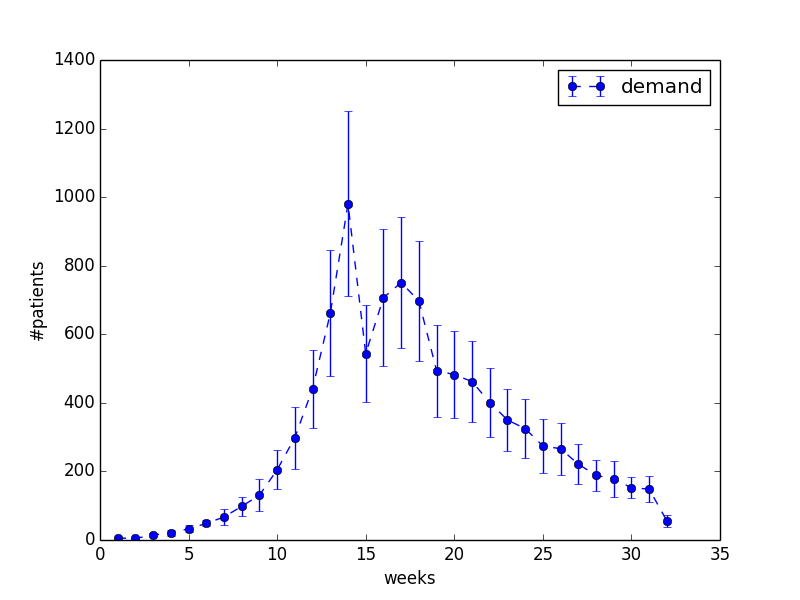
\includegraphics[width=0.4\textwidth]{figs/plot_demand.png}
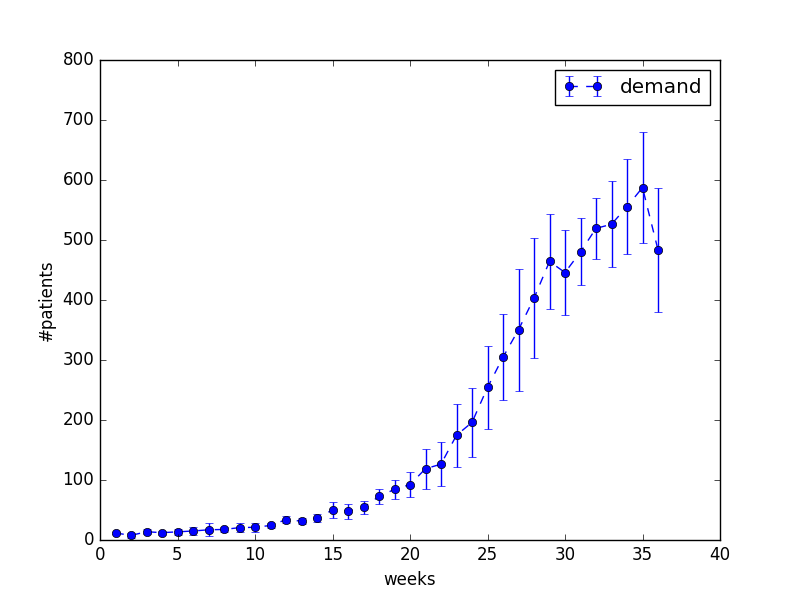
\includegraphics[width=0.4\textwidth]{figs/plot_demand_SL.png}
\caption{Total population demand, i.e., $\sum_j p_j(t)$ as a function of time $t$, for
(a) Liberia and (b) Sierra Leone.}
\label{fig:demand-dist}
\end{figure}

\noindent
\textbf{Constructing the population centers $P$, hospital locations $H$ and distance metric $d$.}
Each cell containing population was converted to a point at the geometric centroid of the cell, 
and assigned the population of the cell; $P$ denotes the set of all such cells.
This process introduces a potential error of up to 700 meters, as the 
population center in any given cell may be near one of the edges or corners, rather than at the 
center as assumed. This error should be random and we do not expect it to significantly affect our placement. 

In order to construct the set $H$,
we restricted candidate supply points to areas with known healthcare facilities. 
It is thought that the Treatment Centers may share common resources with existing clinics, and it may be easier for locals to find the ETCs if they are located near an existing well-known hospital. Also, the areas are likely highly accessible most and should have stable power and clean water. The healthcare facilities are well distributed in populated areas and we do not consider this restriction a limitation to the model. 
The road network of Sierra Leone was sourced from OpenStreetMap,
while the road network of Liberia was derived from spatial data from the Liberian Institute of Statistics and Geo-Information Services (LISGIS) Etherton, 2014). The LISGIS roadmap offers a significant advantage in that it is contiguous, while the OpenStreetMap network has thousands of disconnected edges. Since these segments are disconnected from the central network, individuals on these roads are incapable of ever reaching any facilities and are ignored by our model. In order to account for this in Sierra Leone we manually connected the edges by tracing aerial photography. The use of the LISGIS map of Liberia spared us this effort. The river network was also modelled as it is thought to be a primary means of transportation for some remote jungle regions. It is thought that use of flat-bottom boats makes most of these rivers navigable, and indeed it seems that several communities which appear on LandScan are totally cutoff from the rest of the nation unless the river network is taken into account. As with the road network, the OpenStreetMap version was extremely detailed but featured disconnected segments which prevented population nodes from reaching the ETCs. Instead the less detailed but contiguous river map provided by DIVA-GIS was used \cite{DIVA}. The road and river networks were then combined into a single travel network used for the analysis. Travel speeds were estimated using OpenStreetMap speed limit data. 
Using ArcGIS 10.1 SP1, we stitched together the road and river networks to create a single travel network, then placed the weighted demand and supply points on network edge nearest to them. We then created an origin-destination cost matrix representing travel time from all demand points to all candidate supply points.
\red{citations for some things above}


\noindent
\textbf{Datasets.}
\red{Complete description of these}
Using the above models, we construct three different input instances for \red{Liberia},
referred to as datasets A, B, and C. 
We denote the population demands at a center $j\in P$ in these three instances
by $p_j^A$, $p_j^B$ and $p_j^C$, respectively.
These correspond to three different times during the duration of the outbreak
$A$ denotes the instance at time $t=0$---this
corresponds to the pre-outbreak phase, and 
we assume that any member of the population is equally likely to become infected.
Therefore, $p^A_j$ just corresponds to the population demand at center $j$.
The instance $B$ corresponds to the state at an early stage of the outbreak,
and $p^B_j$ denotes the incidence rates at center $j$ at this time.
Instance $C$ represents the state towards the end of the outbreak,
and $p^C_j$ is the cumulative number of infections at $j$.


%\begin{table}[ht]
%\caption{Summary of datasets and parameters}\label{table:parameters}
%\centering
%\begin{tabular}{cl}
%\toprule
%\multicolumn{2}{c}{Datasets} \\\midrule
%A & Demand is based on LandScan population only\\
%B & Demand based on real 2014-12-05 cases (5 replicates)\\
%C & Demand based on real 2015-04-12 cases (5 replicates)\\\midrule
%\multicolumn{2}{c}{Number of facilities ($k$)} \\\midrule
%k & 16, 20, 24\\\midrule
%\multicolumn{2}{c}{Distance to facility ($r$)} \\\midrule
%$r$ & 0.5, 1, 1.5, 2, 2.5, 3, 3.5 \textcolor{red}{hours} \\\midrule
%\multicolumn{2}{c}{Planning times ($T$): time at which ETU placement is done} \\\midrule
%$T$ & Onset of Epidemic, 2014-12-05, 2015-04-12 \\\midrule
%\multicolumn{2}{c}{Deployment Times} \\\midrule
%$T$ & All on onset, all at ($T1$), all at ($T2$), $\frac{1}{2}$ at onset and 
%$\frac{1}{2}$ at ($T1$), $\frac{1}{2}$ at onset $\frac{1}{4}$ at T1 and $\frac{12}{3}$ at T2 \\\midrule
%\end{tabular}
%\end{table}





%Specific experiments:
%\begin{enumerate}
%\item
%Plot $k$-median cost vs ($k$-center radius) $r$, for each dataset and each deployment time $T$.
%\item
%Some choices of $r$ might not be feasible for covering the entire population. In this
%case, plot the uncovered population vs $r$, for each dataset and each planning time $T$.
%\item
%For the optimal assignment corresponding to a choice of time $T$, plot the
%above curves for other times. This will quantify how the planning done at
%some time works at other times.
%\end{enumerate}


\subsection*{Our algorithms}

\noindent
\textbf{Background.}
The \probstatic{} and \probinc{} problems are both NP-hard, in general, making them hard to solve optimally,
especially on instances of the scale we study here.  We first summarize the key results on optimizing
such objectives, before presenting the algorithms we use.
Charikar, Guha, Tardos, and Shmoys \cite{charikar_kmed} first gave a $6\frac{2}{3}$-approximation algorithm for $k$-median by an LP-rounding algorithm. After a series of improvements, Arya et. al. \cite{arya} introduced a local-search-based $(3+\epsilon)$-approximation algorithm. Recently, Li and Svensson \cite{li_svensson} give a breakthrough result stating that, given any $\alpha$-approximate solution to the $k$-median problem using $k+O(1)$ facilities, one can still transform it into an $(\alpha+\epsilon)$-approximate feasible solution in polynomial time. By opening a small constant extra number of facilities, Li and Svensson manage to improve the ratio when rounding the bi-point solution from $3$ to $\frac{1+\sqrt{3}}{2}$. Taking in account the factor of $2$ when constructing the bi-point solution, this is a $(1+\sqrt{3}+\epsilon) \approx (2.73+\epsilon)$-approximation for the $k$-median problem. The current best known approximation guarantee is $(2.675+\epsilon)$, given by Byrka et. al. \cite{byrka_kmed} In this work, the authors carefully design a set of $9$ different rounding strategies which altogether improve the factor lost when rounding the bi-point solution from $\frac{1+\sqrt{3}}{2} \approx 1.366$ to $1.337$. On the negative side, Jain, Mahdian, and Saberi \cite{jms} showed that the $k$-median is $\mathbf{NP}$-hard to approximate to within $1+2/e \approx 1.735$.

The Capacitated $k$-median (CKM) problem is notoriously difficult to approximate. Recall that, in this problem, each facility $i \in \F$ can only serve at most $c_i$ different clients. There is no known constant approximation algorithm for this problem so far, nor do we know if such an algorithm exists. All known approximation algorithms so far either violate the capacitated constraint or the cardinality constraint. Byrka et. al. give an $O(1/\epsilon^2)$-approximation algorithm by violating the capacity constraint by a factor of $(2+\epsilon)$ in \cite{byrka_ckm}. Recently, Shi Li \cite{li_ckm} shows that there is an $O\left(\frac{1}{\epsilon^2} \log \frac{1}{\epsilon} \right) $-approximation algorithm for the CKM problem if allowed to open $(1+\epsilon)k$ facilities and each facility may be open twice.

The $k$-center problem is NP-hard and is $2$-approximable \cite{book:ws}. Moreover, unless $\mathbf{P} = \mathbf{NP}$, we cannot approximate it to within factor $2-\epsilon$ for any $\epsilon>0$. If we require that some clients may not be open as a center (i.e. $\F \neq \C$), the problem is known as the $k$-supplier problem. It is relatively easy to modify most $2$-approximation algorithms for $k$-center to obtain $3$-approximation algorithms for the case $\F \neq \C$. Also, the lower-bound of $k$-supplier is known to be $3$.

\noindent
\textbf{Our algorithms for the \probstatic{} problem.}
Both the problems we study can be expressed as integer programs, but have millions of variables and
constraints, making them challenging to solve optimally.
We use approximation algorithms that involve first solving a linear relaxation of these programs
(which can be solved in polynomial time), and then carefully rounding the fractional solution 
to a feasible integral solution. We first describe our algorithm for the \probstatic{} problem,
with the $\objcenter$ and $\objmedian$ objectives. We then show how it can be extended to variations,
which relax the problem requirements in various ways.

We start with an integer program for the $\objmedian$ objective---here,
we want open at most $k$ hospital in such a way that the total connection cost is as small as possible. 
The integer programming (IP) formulation for the $k$-median problem is as follows.
\begin{alignat}{2}  
  IP_{\KMED}(\mathbf{p}, P, H, cap, k): \min  &  \sum_{i \in H}\sum_{j \in P} p_j d_{ij} x_{ij} \nonumber\\
    \text{s.t.} & \sum_{i \in H} x_{ij} = 1    &\qquad& \forall j \in P\label{cstr:kmed1} \\
                             &  x_{ij} \leq y_i      && \forall i \in H, j \in P \label{cstr:kmed2}\\
                             &  \sum_{i\in H} y_{i} \leq k      &&  \label{cstr:skmed3}\\
                             & \sum_{j \in P} x_{ij} \leq cap(i)      && \forall i \in O  \label{cstr:kmed-cap} \\
                             & x_{ij},  y_i \in \{0,1\} && \forall i \in H, j \in P \label{cstr:integrality}
\end{alignat}
Here the variable $x_{ij}$ indicates whether population node $j$ will be connected to hospital $i$. The opening variable $y_i$ indicates whether hospital $i$ is opened. The objective function minimizes the total cost of all population nodes (to reach their nearest hospital.) Since the total demand is constant, this is equivalent to minimizing the average cost. Constraint (\ref{cstr:kmed1}) ensures that each population node only pays the cost of one hospital connection in the objective function. Constraint (\ref{cstr:kmed2}) ensures that a population node can only use the cost to hospital $j$ if $j$ is actually part of the solution. Constraint (\ref{cstr:skmed3}) requires that at most $k$ hospitals will be opened.
Constraints (\ref{cstr:kmed-cap}) ensure the capacity of each open facility is satisfied.
Finally, constraints (\ref{cstr:integrality}) ensures that the variables are all integral---it is these constraints
which makes the program very hard to solve.

\noindent
\textbf{Main ideas.}
Let $\LP_{\KMED}(\mathbf{p}, P, H, cap, k)$ denote a linear program, which is obtained by repacing the constraints
(\ref{cstr:integrality}) by $x_{ij},  y_i \in [0,1]$, for all $i, j$.
$\LP_{\KMED}(\mathbf{p}, P, H, cap, k)$ can be solved in polynomial time \cite{gls:book}, and current tools like 
Gurobi.  However, we are left with a fractional solution, e.g., $y_i=0.5$, which does not 
give us a feasible assignment.
Our main idea is to take a solution to $\LP_{\KMED}(\mathbf{p}, P, H, cap, k)$, 
and transform it to a feasible integral solution,
without increasing the cost by ``too much''.
We use a rounding technique from \cite{srin:level-sets}, 
and the minimum cost max-flow, which are summarized below.
Algorithm \ref{algo:kmedstatic} describes \algokmedstatic{}.

\begin{proposition}[\cite{srin:level-sets}]
\label{prop:dep-round}
There exists an algorithm {\sc DepRound}($\mathbf{y}$) which takes as input a vector $\mathbf{y} \in [0,1]^n$ where $\sum_{i=1}^n y_i = k$, and in polynomial time outputs a vector $\mathbf{Y} \in \{0,1\}^n$  with the following properties:
\begin{enumerate}
\item $\Pr[Y_i = 1] = y_i$, for all $i \in [n]$,
\item $\sum_{i=1}^n Y_i = k$ with probability one.
\end{enumerate}
\end{proposition} 

Given a directed graph $G = (V, E)$ with capacity $c_e \in \mathbb{R}^+$ and weight $w_e \geq 0$ on each edge $e \in E$, a source $s$, and a sink $t$. Recall that $f$ is a flow iff it satisfies (1) the capacity constraint: $f_e \leq c_e$ for all $e \in E$ and (2) the conservation constraint: $\sum_{u:(u,v)\in E} f_{(u,v)} = \sum_{u:(v,u) \in E} f_{(v,u)}$ for all $u \in V \setminus \{s, t\}$. The minimum cost max-flow problem is to find a maximum flow $f: E \to \mathbb{R}^+$ from $s$ to $t$ such that the total cost $\sum_e w_e f_e$ is as small as possible.  It is well-known that this problem can be solved efficiently by either linear programming or combinatorial algorithms \cite{flow_book, flow_goldberg, Orlin1997}.


\begin{algorithm}[h]
\caption{$\textsc{Round}\left( \mathbf{y}, r \right)$}
\begin{algorithmic}[1]
\STATE $c \gets +\infty, \mathbf{Y} \gets 0$
\FOR{$z=1,2,\ldots,r$}
	\STATE $\mathbf{Y}' \gets \textsc{DepRound}(\mathbf{y})$
	\IF{$c > $ the cost of opening hospitals in $Y'$}
		\STATE $\mathbf{Y} \gets \mathbf{Y}'$
		\STATE $c \gets $ the cost of $\mathbf{Y}'$
	\ENDIF
\ENDFOR
\RETURN $\mathbf{Y}$
\end{algorithmic} 
\end{algorithm}

\begin{algorithm}[h]
\caption{$\algokmedstatic \left(H, P, \mathbf{p}, w, \ell, r_{\text{depRound}} \right)$}
\label{algo:kmedstatic}
\begin{algorithmic}[1]
\STATE \red{correct the algorithm description}
\STATE $\mathbf{y} \gets \LP_{\CAPKMED}(\mathbf{p}, cap(u), k)$
\STATE $\mathbf{Y} \gets \textsc{Round}\left( \mathbf{y}, r_{\text{depRound}} \right)$
\STATE $O \gets \{i \in H: Y_i = 1\}$
\STATE Let $V = \{v_s, v_t\} \cup P  \cup O$. Construct a graph on $V$ as follows.
\STATE Create an edge $(v_s, j)$ for each $j \in P$ with capacity $c_{(v_s, j)} = p_j$ and weight $w_{(v_s, j)} = 0$.
\STATE Create an edge $(j, i)$ for each $j \in P$ and $i \in O$ with capacity $c_{(j, i)} = +\infty$ and weight $w_{(j, i)} = d_{i, j}$.
\STATE Create an edge $(i, v_t)$ for each $i \in O$ with capacity $c_{(i, v_t)} = cap(u)$ and weight $w_{(i, v_t)} = 0$.
\STATE Find the minimum cost max-flow $f$ from $v_s$ to $v_t$. For each $j \in P$ and $i \in O$, assign $f_{j,i}$ patients from node $j$ to hospital $i$.
\end{algorithmic} 
\end{algorithm}

\begin{theorem}
\label{theorem:kmedstatic}
\red{Algorithm \algokmedstatic{} gives a ... approximation}
\end{theorem}

\noindent
\textbf{Extensions for other variations.}
We study several variations of the \probstatic{} and \probinc{} problems, and our algorithms have the same
general structure as \algokmedstatic{} above. For brevity, we summarize the main changes in the algorithms here,
and present the complete details in the Supplementary Information.
\begin{enumerate}
\item
Optimizing the $\objcenter$ objective: 
\item
Minimizing cost of closest clients: 
we only study fractional solutions to this problem, which can be computed using a linear program.
We change the objective in $\LP_{\CAPKMED}(\mathbf{p}, cap(u), k)$
to $\sum_{i \in H, j \in P: w_{ij} \leq D} p_j d_{ij} x_{ij}$,
and add constraints $\sum_{i \in H: w_{ij} \leq D} x_{ij} \leq 1$, and
$\sum_{j \in P} \sum_{i \in H: w_{ij} \leq D} p_j x_{ij} \geq  (1-\epsilon) \left( \sum_{j \in P}p_j \right)$.
\item
Maximizing number of close clients:
for this variation as well, we only study the fractional solution. This can be computed by changing the
$\LP_{\CAPKMED}$ by maximizing $\sum_{j\in P}\sum_{i\in H} x_{ij}p_j$, and setting $x_{ij} = 0$,
for all $i\in H, j\in P \mbox{ with }d_{ij}>D$.
\end{enumerate}

\noindent
\textbf{Kernel facilities.}
Both types of objectives assume the number of facilities, $k$, is known in advance.
In real scenarios, facilities may be placed over time in incremental steps or stages, the final number of which may not be known. In this case given, say, 5 facilities to start with, we don't just want to find the best solution using 5 facilities, but one that would continue to give good solutions if more facilities are added in future.
To this end we introduce the notion of a ``kernel''. 
Roughly speaking, a kernel is a set of \textit{important} facilities that appear in many different solutions regardless of the value of $k$ chosen. They also have the stability property that larger kernels are always supersets of all smaller kernels. This is rarely the case when using $k$-median solutions directly.

Our algorithm \algokernelkmed{} for finding a kernel set involves the following steps.
\begin{enumerate}
\item
Let $0 < r \leq n$ be some parameter. 
\item
We solve the $k$-median problem with $k = 1, 2, \ldots, r$ using population demands. 
\item
For each facility $i \in H$, we record the frequency that $i$ appears in our $r$ solutions.
\item
We define the $\ell$-kernel as the $\ell$ facilities which have the highest frequencies. 
\end{enumerate}



\subsection*{Algorithm for the \probinc{} problem}
In this section, we consider the setting where facilities might be deployed incrementally, with a fixed capacity. We consider a given schedule $t_0, t_1, \ldots, t_m$, which denote the discrete times at which we want to monitor the epidemic. At time $t_u$, we let $k_u \geq 0$ denote the number of new facilities with uniform capacity $cap_u \geq 1$ that can be deployed. We also $\mathbf{p}(t_u)$ be the demand vector at time $t_u$. In our experiments, $t_1, t_2, \ldots, t_m$ are equidistant and corresponding to the times after $1$ week, $2$ weeks, and so on. Our method \textsc{OnlineKMed} starts with an initial
deployment of $k_0$ facilities at time $t_0$, based on the population density, and at each subsequent time $t_u$ with $u > 0$, it uses the current infection rates to determine the locations where $k_u$ additional facilities could be deployed, \emph{without altering the locations of facilities already deployed}. Let $O_u$ denote the set of open hospital at time $t_u$. We require that $O_0 \subseteq O_1 \subseteq O_2 \ldots \subseteq O_m$.

Let us consider any time $t_u$ where $u > 0$. Let $C_{u-1}$ denote the total capacities of all hospital up to time $t_{u-1}$. The first question is ``how should we determine the number $k_u$ of new hospitals to be built?'' In practice, there are two main factors for estimating parameter $k_u$: (1) our current budget and (2) the forecasted demand vectors $\mathbf{p}(t_v)$ for a few next time points $\{t_v: v \geq u\}$. Indeed we want to cover as many population nodes as possible; however, the total opening cost will have to be bounded by some given budget.

Now suppose we know the value of $k_u$. Then the maximum number of patients who can be served is $C_u = C_{u-1} + k_u \times cap_u$. We have two cases:
\begin{itemize}
	\item Case $C_u \geq |\mathbf{p}(t_u)|_1$: it is possible to serve all patients at time $t_u$. We solve the corresponding capacitated $k$-median instance with the set $O_{u-1}$ being opened and obtain the solution $O_u$. Now the optimal assignment of patients to open facilities in $O_u$ can be easily found by solving a minimum cost max-flow problem.
	
	\item Case $C_u < |\mathbf{p}(t_u)|_1$: it is impossible to serve all patients at time $t_u$. We suggest the following policy. We sort all patients (recall that the node $j \in P$ has $p_j(t_u)$ patients at time $t_u$) in decreasing order of distance to the nearest hospital in $H$. Let $S_u$ be the set of the top $|\mathbf{p}(t_u)|_1 - C_u$ patients in this list. We refer to $S_u$ as the set of ``outliers'' at time $t_u$. We shall need some alternative treatment for the people in $S_u$. Then we exclude $S_u$ from $P$ to obtain a new demand vector $\mathbf{p}'(t_u)$ such that $|\mathbf{p}'(t_u)|_1 = C_u$. The problem can now be solved as in the first case.
	
\end{itemize}





Consider any time point $t_u$. Recall that $k = k_u$ is the number of additional hospitals to be built, $O = O_{u-1}$ is the set of open hospitals up to this time, $\mathbf{p}$ and $P$ are the demand vector and population set after excluding the outliers respectively, and $c = cap_u$ is the capacity for all hospitals to be opened at time $t_u$. For each $i \in O$, recall that $cap(i)$ is the (fixed) capacity of hospital $i$ which was chosen when building $i$. The LP relaxation for the capacitated $k$-median problem at time $t_u$ is as follows.

\begin{alignat}{2}  
  \LP_{\CAPKMED}(O, \mathbf{p}, P, c, k): \min  &  \sum_{i \in H}\sum_{j \in P} p_j d_{ij} x_{ij} \nonumber\\
    \text{s.t.} & \sum_{i \in H} x_{ij} = 1    &\qquad& \forall j \in P  \\
                             &  x_{ij} \leq y_i      && \forall i \in H, j \in P \ \\
                             & \sum_{j \in P} x_{ij} \leq cap(i)      && \forall i \in O  \label{cstr:kmed3} \\
                             & \sum_{j \in P} x_{ij} \leq c      && \forall i \in H \setminus O  \label{cstr:kmed4} \\
                             & y_i = 1    && \forall i \in O  \\
                             &  \sum_{i\in H} y_{i} \leq |O|+k_u      &&  \\
                             & x_{ij},  y_i \in [0,1]&& \forall i \in H, j \in P.\nonumber
\end{alignat}
The constraints (\ref{cstr:kmed3}) and (\ref{cstr:kmed4}) make sure that no hospital will serve more patients than its capacity. 


We are now ready to describe our main algorithm.
\begin{algorithm}[h]
\caption{$\textsc{OnlineKMed} \left(H, P, \mathbf{p}, w, \ell, r_{\text{kernel}}, r_{\text{depRound}} \right)$}
\begin{algorithmic}[1]
\STATE Time $t_0$: compute the kernel $O_0 \gets \textsc{KernelKMed}(\ell, r_{\text{kernel}})$
\FOR{each $t_u$ where $u = 1,2,\ldots, m$}
	\STATE Choose $k_u$ and $cap(u)$ based on the current budget and the forcasted demand vector $\mathbf{p}(t_u)$
	\STATE Compute the set of outliers $S_u$ and the updated demand vector $\mathbf{p}'(t_u)$ after excluding the nodes in $S_u$
	\STATE $\mathbf{y} \gets \LP_{\CAPKMED}(O_{u-1}, \mathbf{p}'(t_u), P \setminus S_u, cap(u), k_u)$
	\STATE $\mathbf{Y} \gets \textsc{Round}\left( \mathbf{y}, r_{\text{depRound}} \right)$
	\STATE $O_t \gets \{i \in H: Y_i = 1\}$
	\STATE Let $V = \{v_s, v_t\} \cup (P \setminus S_u) \cup O_t$. Construct a graph on $V$ as follows.
	\STATE Create an edge $(v_s, j)$ for each $j \in P \setminus S_u$ with capacity $c_{(v_s, j)} = p_j'(t_u)$ and weight $w_{(v_s, j)} = 0$.
	\STATE Create an edge $(j, i)$ for each $j \in P \setminus S_u$ and $i \in O_t$ with capacity $c_{(j, i)} = +\infty$ and weight $w_{(j, i)} = d_{i, j}$.
	\STATE Create an edge $(i, v_t)$ for each $i \in O_t$ with capacity $c_{(i, v_t)} = cap(u)$ and weight $w_{(i, v_t)} = 0$.
	\STATE Find the minimum cost max-flow $f$ from $v_s$ to $v_t$. For each $j \in P \setminus S_u$ and $i \in O_t$, assign $f_{j,i}$ patients from node $j$ to hospital $i$.
\ENDFOR
\end{algorithmic} 
\end{algorithm}






% Results and Discussion can be combined.
\section*{Results}

We start with different variations of the \probstatic{}: we compare the two objectives
$\objcenter$ and $\objmedian$, and study the effects of relaxing various constraints in the problem.
Then, we consider the more realistic incremental version of the problem.

\subsection*{Individual vs social cost}
The $\objcenter$ objective models the individual cost, whereas the $\objmedian$ objective
is a better model of the social cost. 
Figure \ref{fig:kmed_vs_ksup} shows a comparison between these two objectives in Dataset A, as a function of
$k$, the number of facilities.
As one might expect, there is a significant tradeoff between these two objectives---the $\objcenter$ value
is almost three times the $\objmedian$ value for most values of $k$ for Sierra Leone; it is even higher for Liberia.
If there are difficult-to-reach areas (with high travel cost from other areas),
the $\objcenter$ can have a large value; the $\objmedian$ value might still be small if there are only
few such areas.  Therefore, these objectives need to be considered carefully during the planning process.

Next, we study if ignoring the connection costs for a small fraction of people can lead to a
significant improvement in the connection cost of the remaining population.
To explore this question, we develop two modified formulations of the \probstatic{} problem with the
$\objmedian$ objective.
First, how well does the $\objmedian$ solution do at minimizing the travel time of some fraction of 
the population of the population? 
Secondly, how well does the $\objmedian$ solution
do at maximizing the amount of people which obtain a specific travel time? 




\begin{figure}[h]
\centering
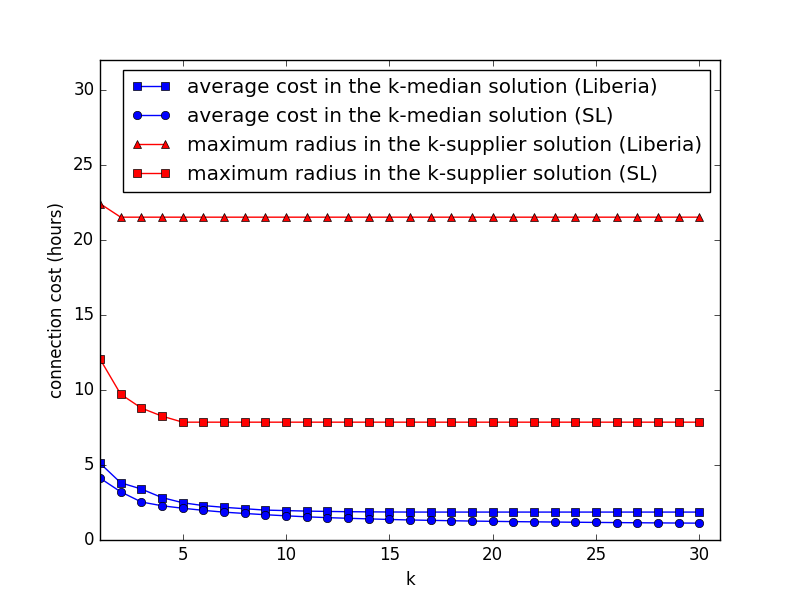
\includegraphics[width=0.5\textwidth]{new_figs/plot_A_kmed_vs_ksup.png}
\caption{Comparisons between the $k$-median and $k$-supplier objective functions for Dataset A.}\label{fig:kmed_vs_ksup}
\end{figure}


\subsubsection*{Minimizing cost of closest clients}
Recall that the goal here is:
given a cutoff distance $D$ and fraction $\epsilon$, minimize the average cost of the 
closest $(1-\epsilon)n$ clients subject to the constraint that those clients are all 
within distance $D$ of an open facility. 
In order to understand the impact of $D$ and $\epsilon$ in such a formulation, we compare the
fractional solution for this problem (by solving an LP), with the $\objmedian$ solution.
Figure \ref{fig:kmed_vs_LP1} shows the results for $D=6$ hrs and varying 
values of $\epsilon$, along with the solution to the $\objmedian$ objective (without any bound on $D$). 
For each value of $\epsilon$, we compared the cost of the top $(1-\epsilon)n$ clients 
(referred to as ``good'' clients) in the LP solution, against the cost of the top $(1-\epsilon)n$ 
clients in the ordinary $k$-median solution.
\red{clarify the previous sentence}
We observe that solutions allowing for violations only marginally 
improve the travel time of the top $(1-\epsilon)n$ clients over that of the $\objmedian$ solution.
These results indicate that, in practice, the ordinary $k$-median solution is already quite good with respect to 
these constraints, when $k$ is not too small.


\begin{figure}[h]
  \centering % left bottom right top
	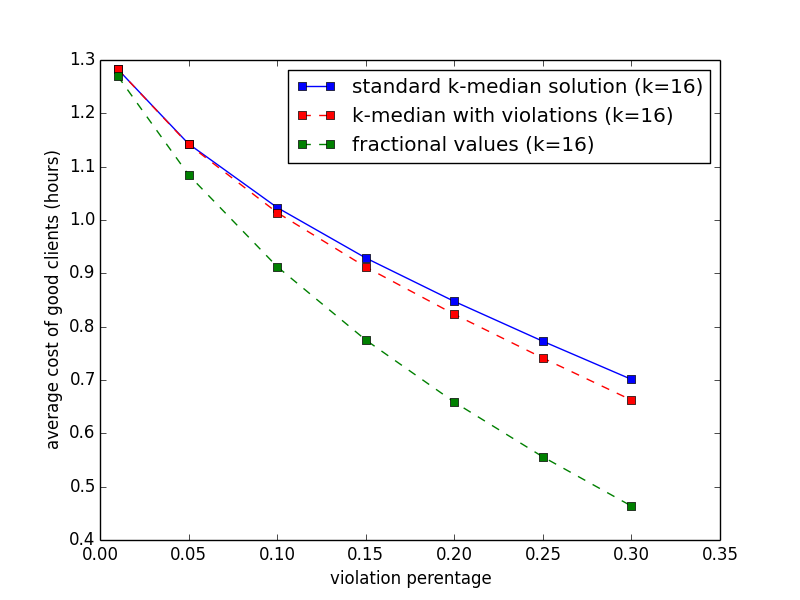
\includegraphics[width=0.48\textwidth]{figs/plotA16_violation.png}
	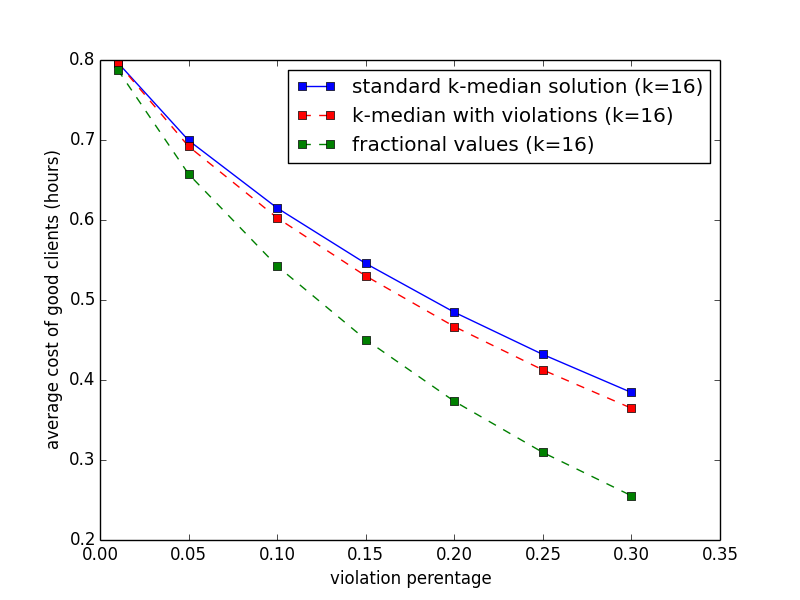
\includegraphics[width=0.48\textwidth]{figs/plotB16_violation.png}
\caption{Average cost of top $(1-\epsilon)n$ clients, for $k$-median solution and LP1 solution (fractional and best integral solution found) on Dataset A (left) and B (right). (Liberia)} 
	\label{fig:kmed_vs_LP1}
\end{figure}


\subsubsection*{Maximizing number of close clients}
Recall that here the goal is to maximize the number of clients which have a hospital within a given bound $D$.
Again, we study how the solution to the $\objmedian$ objective compares with a solution to such a formulation.
We solve an LP for this formulation, 
for $D$ varying from 2 to 7 hours, using $k=16$. We then take the solution to ordinary $k$-medain for $k=16$, 
and measure how many clients lie within distance $D$ for each value. 
Figure \ref{fig:LP2_AB} shows that the $k$-median solution comes quite close to the fractional solution.
These results again suggest that the $k$-median solution is already quite robust, in that it already does 
a good job maximizing the number of clients within distance $D$, for many values of $D$ simultaneously. 
Our conclusion in this subsection is that it is only marginally beneficial to exclude any of the population as outliers. The ordinary $k$-median problem already yields a good quality solution. 

\begin{figure}[h]
  \centering % left bottom right top
    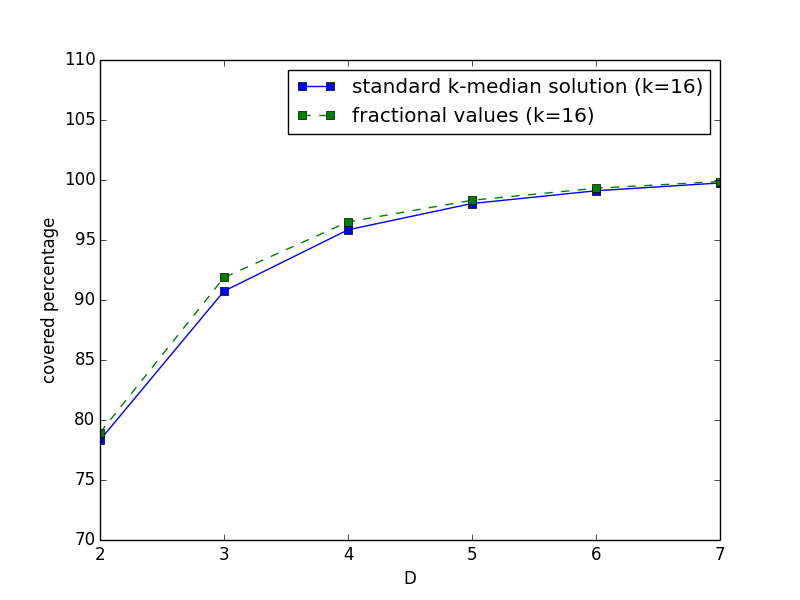
\includegraphics[width=0.4\textwidth]{figs/plotA16_min_violation.png}
	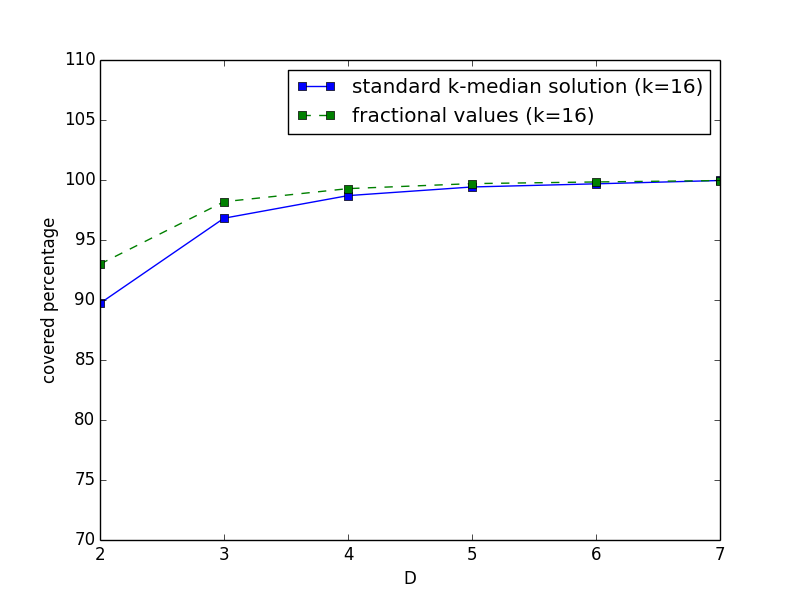
\includegraphics[width=0.4\textwidth]{figs/plotB16_min_violation.png}
\caption{Our results of solving LP2 for Dataset A (left), and B (right). (Liberia)} 
	\label{fig:LP2_AB}
\end{figure}



\subsection*{Kernel facilities}
We run algorithm \algokernelkmed{} on datasets A and B \red{(averaged across all subinstances, $r = 30$)}.
Figure \ref{fig:coreset_A_and_B} shows the frequencies of facilities, sorted in decreasing order.
The figure shows that there are many facilities which occur in most of the solutions, and many facilities which are rarely used in any solution.
Recall that we define the $\ell$-kernel as the $\ell$ facilities which have the highest frequencies. For example, the $10$-kernel for Dataset A is strong, as all its facilities occur in at least $90$\% of the solutions. Dataset B has weaker kernels, possibly because it is an average over multiple possible demand sets. Comparing the kernels of Datasets A and B, there is no apparent correlation. Our explanation is that the most useful facilities for the population data are spread out across the country.


\begin{figure}[h]
  \centering % left bottom right top
    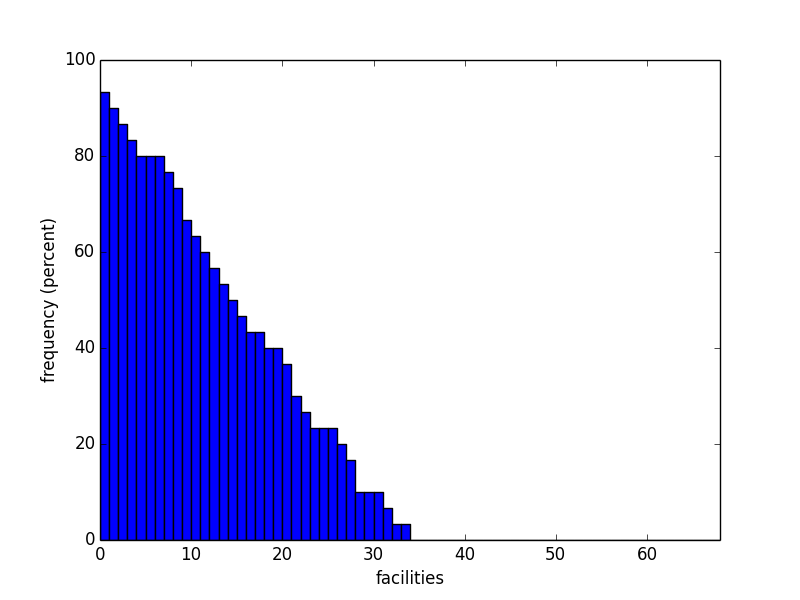
\includegraphics[width=0.4\textwidth]{figs/coresetA.png}
        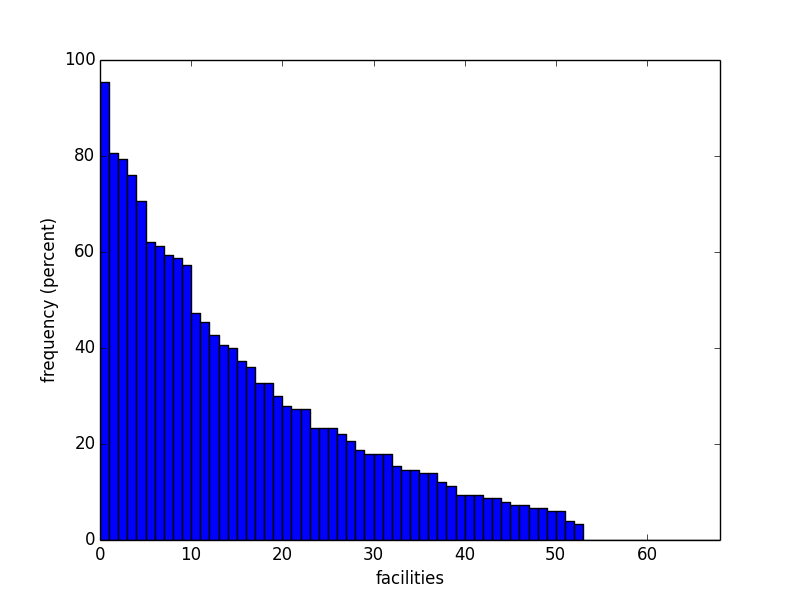
\includegraphics[width=0.4\textwidth]{figs/coresetB.png}
\caption{Facility frequencies for Dataset A (left) and Dataset B (right), sorted by frequency. (Sierra Leone)}
        \label{fig:coreset_A_and_B}
\end{figure}



\begin{figure}[h]
  \centering
    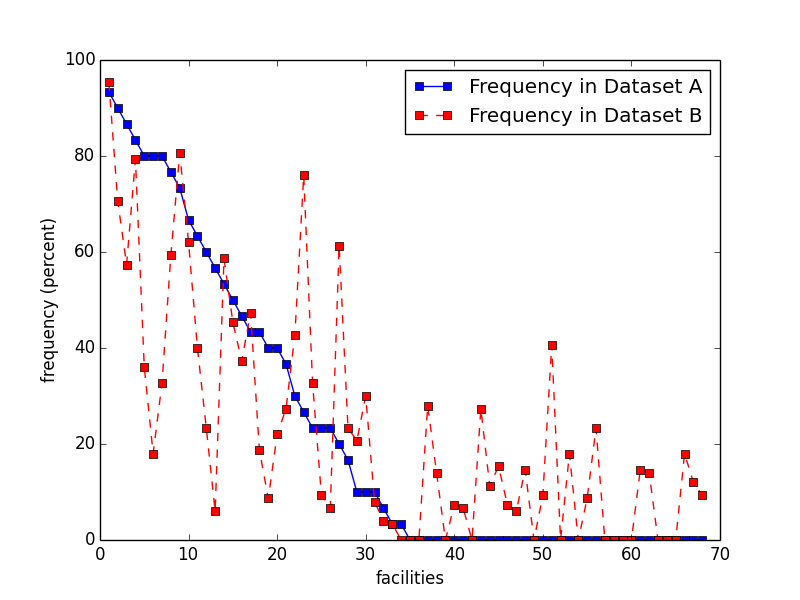
\includegraphics[width=0.4\textwidth]{figs/coreset_AB.png}
    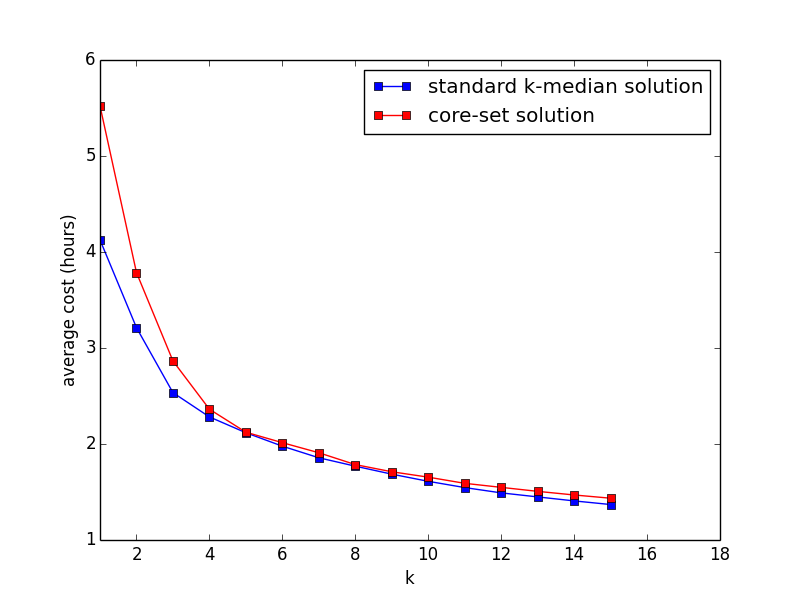
\includegraphics[width=0.4\textwidth]{figs/core_only.png}
\caption{
(a) Facility frequencies compared between Dataset A and B.
(b) Performance of the optimal $k$-median solution vs. the kernel solution of size $k$, in dataset A. (Sierra Leone)
} 
        \label{fig:coreset_AB}
\end{figure}





\subsection*{Importance of forecasting}
The epidemic dynamics drives the demand for healthcare resources, and it seems
likely that planning using forecast demands would give improvements over not
considering such information at all. At the same time, there is uncertainty
in forecasts using all current methodologies, especially at a high
spatio-temporal scale \cite{chakraborty:sdm14}.
In order to evaluate the effect of forecasting,
we consider solutions for instance $C$ computed in three different
ways: (1) the optimum solution, denoted by $OPT_C$;
(2) the solution computed by using $p^B_j$ as the demands;
and (3) the solution computed by using $p^A_j$ as the demands.
Figures \ref{fig:ABC_L} and \ref{fig:ABC_L} show this comparison for several values of $k$.

%In the $k$-median problem, we examine demands at a single time step and find an optimal solution. But as the outbreak evolves, the demands shift and the solution will no longer be optimal. In the following experiment, we suppose that the solution is generated based off of t=0, 1, or 2 data, and then measure how well that solution performs given the t=2 demand. For t=0, this means determining the facility set pre-outbreak, based on population alone. For t=1, this means either waiting until the t=1 time point to determine the facility set, or using accurate modeling to predict the t=1 situation. For t=2, this again means either waiting until t=2 to actually determine the facility set, or using accurate modeling. All 3 of these solutions are then applied to the t=2 demand set and the average distance measured. Using the t=2 data will by definition give the best-possible solution, so the interest is in comparing the t=2 solution against the t=0 and 1 solutions. Figure \ref{fig:ABC} shows this comparison for several values of $k$.


\begin{figure}
    \centering
       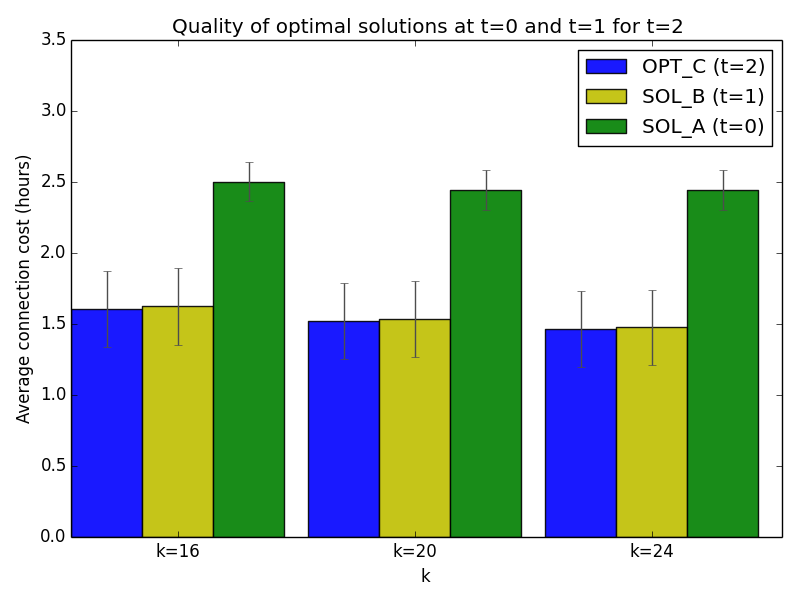
\includegraphics[width=0.40\textwidth]{new_figs/plotABC_L.png}
       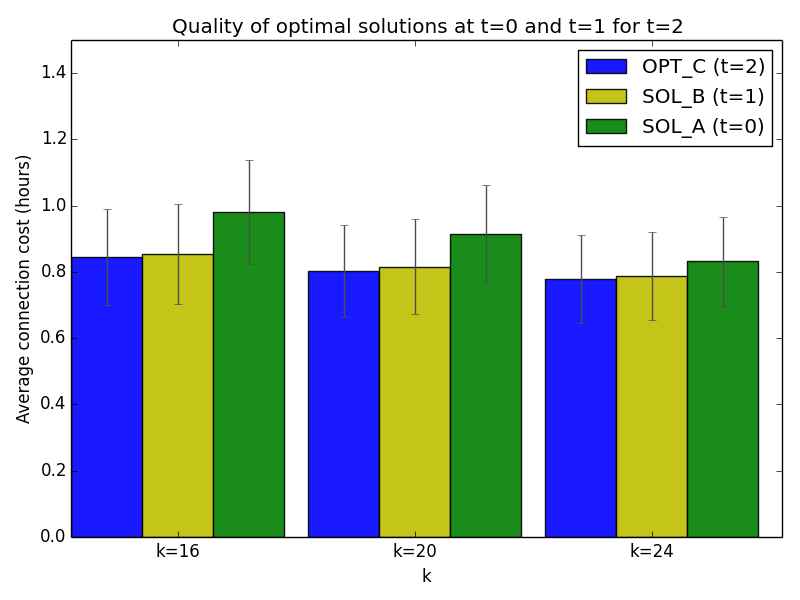
\includegraphics[width=0.40\textwidth]{new_figs/plotABC_SL.png}
    \caption{Quality of the solutions at time $t=0$ and $t=1$ at time $t=2$ for Liberia (left) and Sierra Leone (right). }
\label{fig:ABC_2countries}
\end{figure}

\begin{figure}
    \centering
       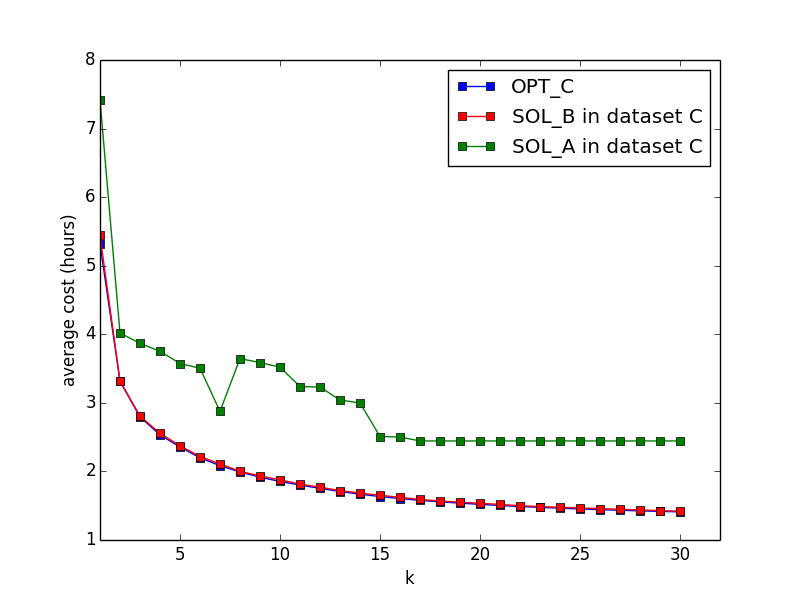
\includegraphics[width=0.40\textwidth]{new_figs/ABC_average_L.png}
       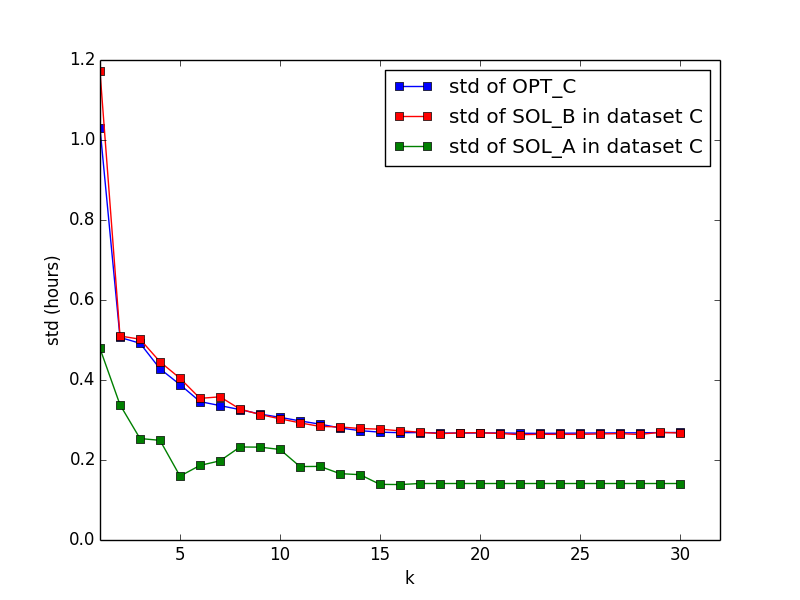
\includegraphics[width=0.40\textwidth]{new_figs/ABC_std_L.png}
    \caption{Compare solutions calculated at each time. (Liberia)}
\label{fig:ABC_L}
\end{figure}

\begin{figure}
    \centering
       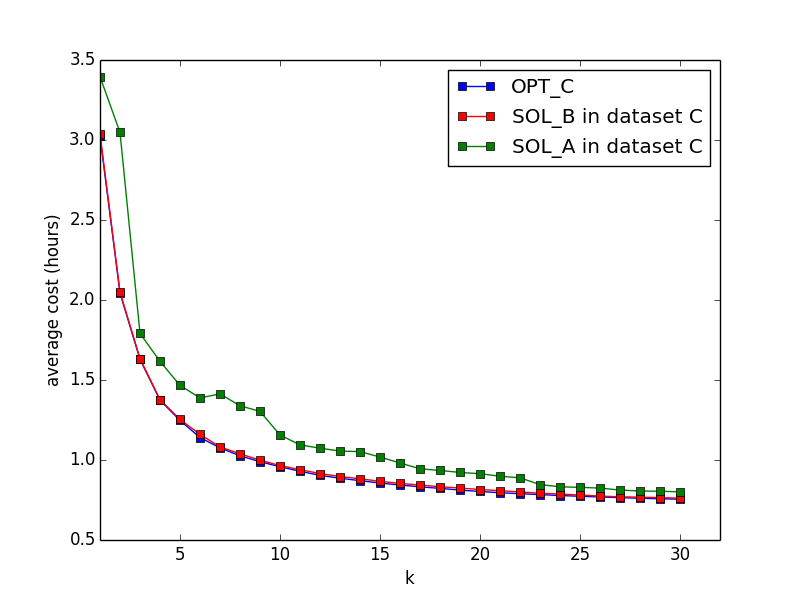
\includegraphics[width=0.40\textwidth]{new_figs/ABC_average_SL.png}
       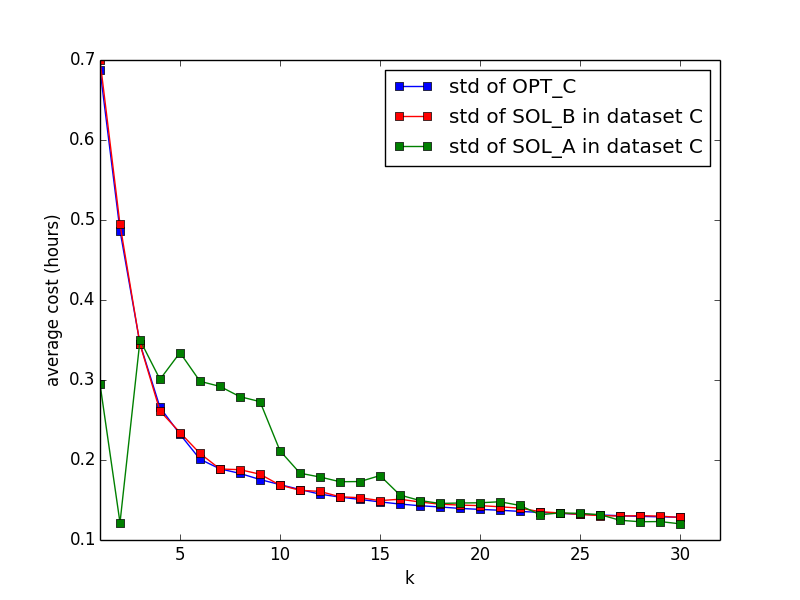
\includegraphics[width=0.40\textwidth]{new_figs/ABC_std_SL.png}
    \caption{Compare solutions calculated at each time. (Sierra Leone)}
\label{fig:ABC}
\end{figure}

\noindent
Our main observations here are
\begin{itemize}
\item
We find that the solution $p^B_j$ computed using demands from B is significantly better than the
solution $p^A_j$ computed using the demands from instance A. For instance, as Figure \ref{fig:ABC_L}
shows an almost 40\% reduction in the average cost objective, for $k=16$ facilities.
Indirectly, this suggests that instead of using static population demands, if we were able to obtain 
forecasts, this would give much better solutions.
%Deciding the facility locations by taking forecasted incidence rates can significantly
%improve the quality of the solution, especially when the number of facilities is low.
%For instance, if 5 facilities are to be placed, using the forecasted demand can give
%close to 10-15\% reduction in the average travel time, compared to solutions that do
%not take forecasts into account.
%With the new dataset B (t=1), t=1 behaves very similarly to t=2. There is some difference between t=0 and t=2, which vanishes as $k$ increases. ``Does the small difference between T1 and T2 solutions imply that the disease had reached its maximum spatial distribution before exponential growth began?''
\item
The precise benefits from using forecasting are hard to guage without using results from specific
forecasting methods; however, that can bring in additional difficulties relating to the performance of the
forecasting methods themselves. Instead, we examine the effects of uncertainty on demands on the
performance, which give us some insights into how well the forecasting methods should be.
We discuss the effects of uncertainty below for $k=16$ facilities.
\begin{itemize}
        \item We perturb all distances by a random $\delta \in [-1.5, +1.5]$ (hours), 
and solve the $k$-median instances (repeat $20$ times). We find that 15 out of the 16 facilities appear
in the solutions for all the 20 trials.

        \item Repeat the experiment with $\delta \in [-1, +1]$. Result : $15/16$ facilities appear in all $20$ trials; there's one facility appearing in $\approx 80\%$ of the trials.

        \item Perturb each distance $w_{ij}$ by $w_{ij} \gets w_{ij} + \delta w_{ij}$ where $\delta \in [-0.35, +0.35]$. Result : $15/16$ facilities appear in all $20$ trials; there's one facility appearing in $\approx 10\%$ of the trials.
\end{itemize}
\end{itemize}



\subsection*{Performance of a hybrid approach}
We have seen in the last subsection that using a set of facilities completely based on the static population information would be bad as the epidemic spreads in the future. On the other hand, it is crucial to ``pre-open'' a few hospitals to control the disease at the early stage of the epidemic. Here we consider a hybrid approach which opens $\ell$ facilities at timestep $t=0$, and $k-\ell$ additional facilities at timestep $t=2$. This solution will be evaluated on Dataset C.

How should we choose the set of important facilities to pre-open at time $t = 0$? In our below results, this set will be chosen as the $\ell$-kernel in Dataset A (using \textsc{KernelkMed}) with $\ell = 5$ facilities. The results show that once $k$ is a little higher than the kernel size, the solutions obtained are quite good; they are very close to the optimal solutions based entirely on the later time point. Determining the entire solution based on Dataset A on the other hand leaves a significant gap in optimality at a later time point.


\begin{figure}[h]
    \centering
       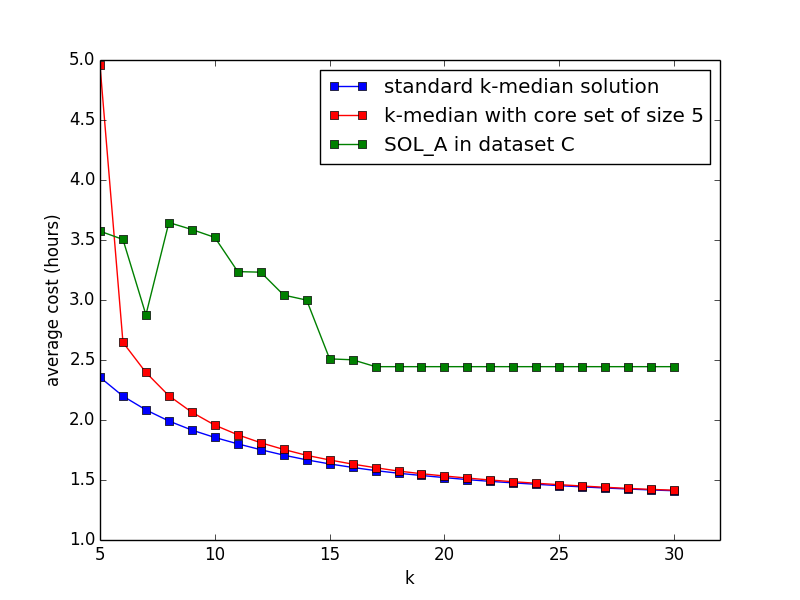
\includegraphics[width=0.40\textwidth]{new_figs/plotC_hybrid_freq_L.png}
       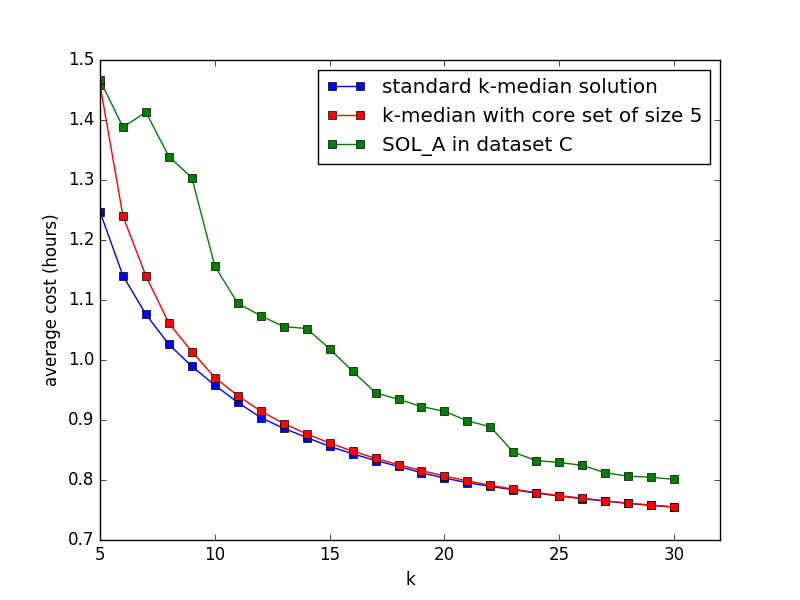
\includegraphics[width=0.40\textwidth]{new_figs/plotC_hybrid_freq_SL.png}
    \caption{Hybrid solutions for Liberia (left) and Sierra Leone (right).}
\label{fig:hybrid}
\end{figure}


\subsection*{Incremental facility location}
\red{this overlaps with the hybrid version above. Maybe merge both?}
In this section, we summarize our numerical results for the incremental hospital location problem. Recall that $t_1, t_2, \ldots$ are the times after $1$ week, $2$ weeks, etc from the start of the epidemic. We exploit the property of kernel facilities in the following manner: for the first $s-1$ time points (weeks), $t_1, \ldots, t_{s-1}$, we only use the kernel with uniform capacity $cap_1$. Starting from time $t_{s}$, we build $k'$ additional hospitals at time points  $t_s, t_{s+w}, t_{s+2w}, \ldots$ for some $w \in \mathbb{N}$. In other words, we are able to build $k'$ additional facilities after every $w$ weeks starting from time $t_s$. These new hospitals will have uniform capacity $cap_2$.


\begin{itemize}
\item
Figure \ref{fig:online1} compares the incremental solution with 
$s=1$, $w=2$, $k=5, k' = 2$, $cap_1 = cap_2 = 100$, with the static fractional solution
(which serves as a lower bound). We find that the solutions are really close, after about 5 weeks.
\item
The performance of the incremental approach depends on the initial capacity, $cap_1$, as shown
in Figure \ref{fig:online2}. If $cap_1$ is too low, this can cause spikes in the average cost
at some subsequent time, when the patient demand peaks.
\item
Another important determinant for the performance of the incremental algorithm is the
number $k'$ of facilities opened at each time. Figure \ref{fig:online3} compares two different
policies, namely (i) one every two weeks, starting at week 10, and
(ii) two each week, starting week 1. As one would expect the former has a much
higher cost, especially in the early stages of the epidemic.
\end{itemize}

\begin{figure}[h]
  \centering % left bottom right top
    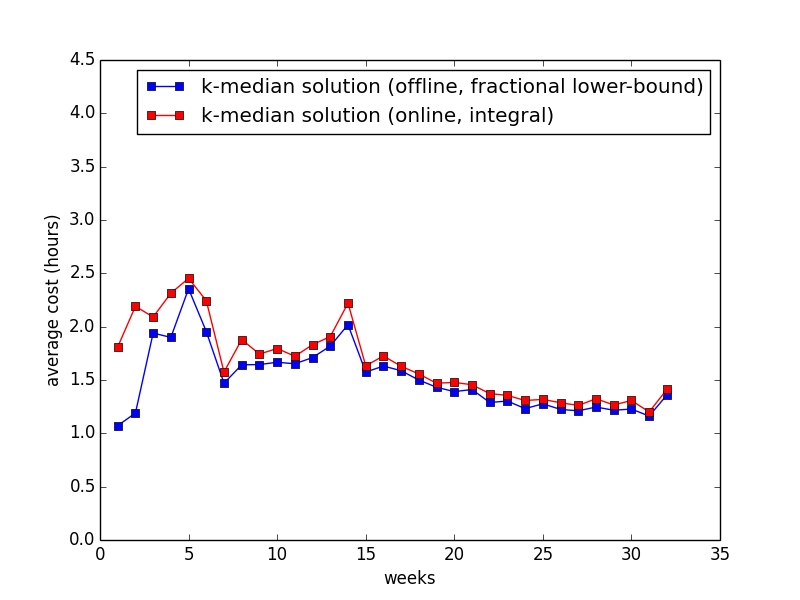
\includegraphics[width=0.30\textwidth]{figs/plot_kmed_CAP100.png}
    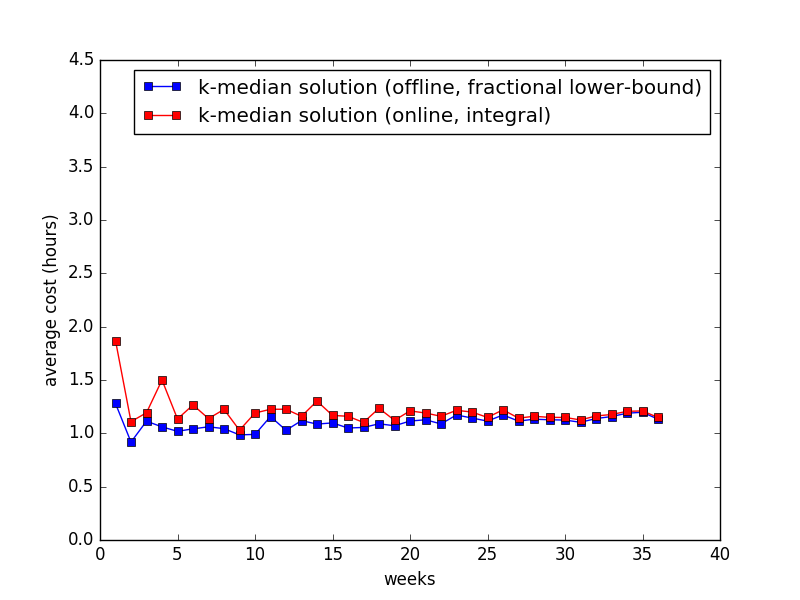
\includegraphics[width=0.30\textwidth]{figs/plot_kmed_CAP100_SL.png}
    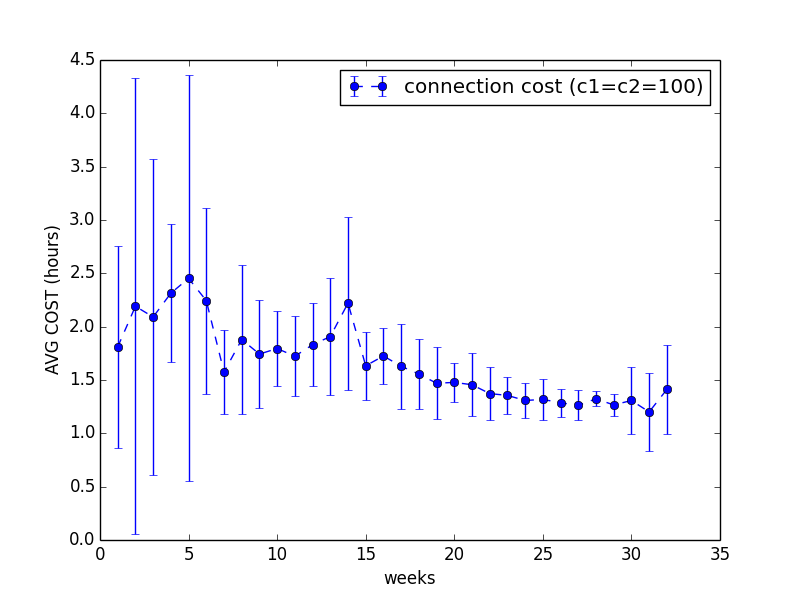
\includegraphics[width=0.3\textwidth]{figs/plot_online_cap100.png}
    \caption{Comparing the static and incremental strategies for
$s=1$, $w=2$, $k=5, k' = 2$, $cap_1 = cap_2 = 100$ for
(a) Liberia, and (b) Sierra Leone.
The variance in the solution costs over multiple iterations is shown in (c).}
\label{fig:online1}
\end{figure}

\begin{figure}[h]
  \centering % left bottom right top
    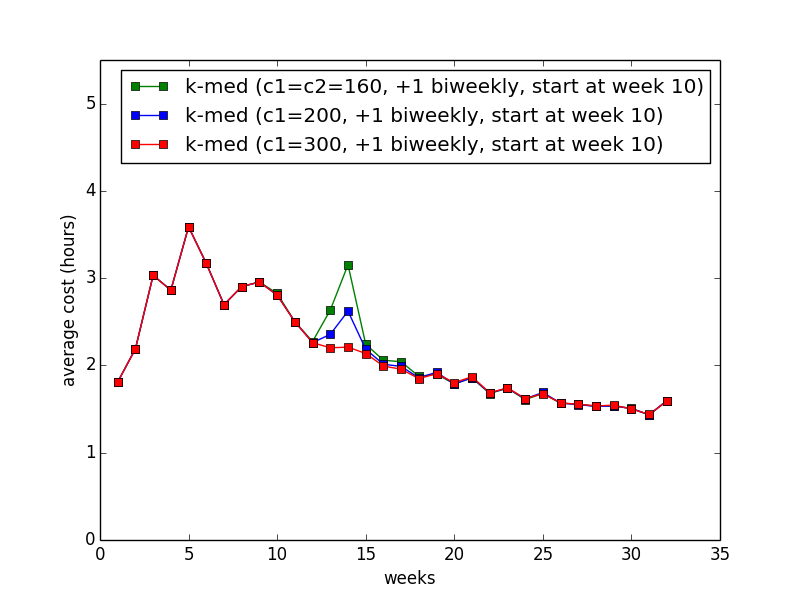
\includegraphics[width=0.45\textwidth]{figs/plot_kmed_c1.png}
    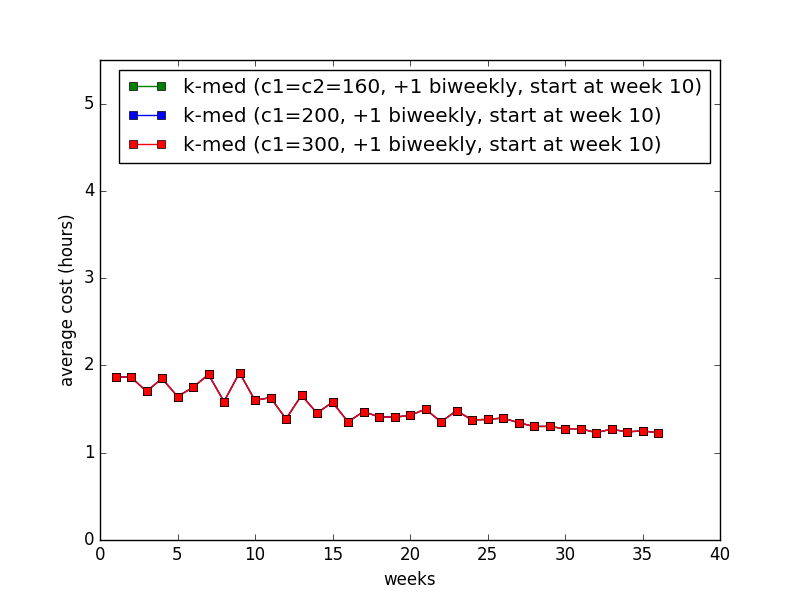
\includegraphics[width=0.45\textwidth]{figs/plot_kmed_c1c2_SL.png}
    \caption{Effect of the initial capacity $cap_1$ on the incremental solution, with
parameters $s = 10, w = 2, k' = 1, cap_2 = 160$, for (a) Liberia, and (b) Sierra Leone.}
\label{fig:online2}
\end{figure}

\begin{figure}[h]
  \centering % left bottom right top
    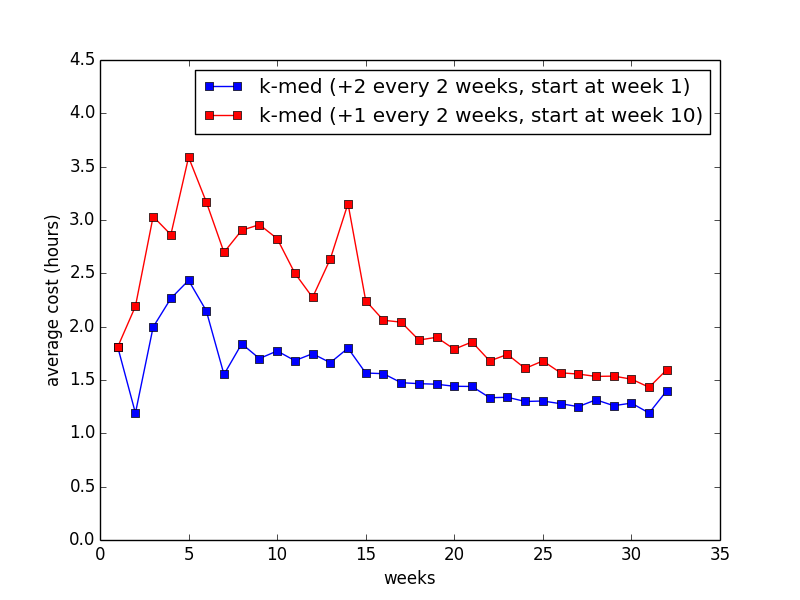
\includegraphics[width=0.45\textwidth]{figs/plot_kmed_CAP160_s1_s10.png}
    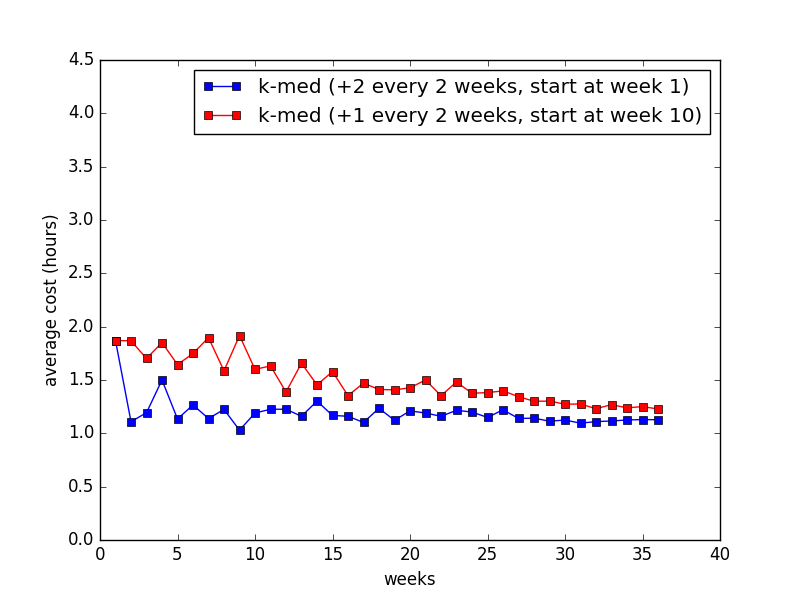
\includegraphics[width=0.45\textwidth]{figs/plot_kmed_CAP160_s1_s10_SL.png}
    \caption{Two different opening policies, with kernel size = $5$, for
(a) Liberia and (b) Sierra Leone.}
\label{fig:online3}
\end{figure}



%%\section{The Incremental facility location problem}
%%%\subsection{Incremental facility location}
%\label{sec:incremental}

In this section, we consider the setting where facilities might be deployed incrementally, with a fixed capacity. We consider a given schedule $t_0, t_1, \ldots, t_m$, which denote the discrete times at which we want to monitor the epidemic. At time $t_u$, we let $k_u \geq 0$ denote the number of new facilities with uniform capacity $cap_u \geq 1$ that can be deployed. We also $\mathbf{p}(t_u)$ be the demand vector at time $t_u$. In our experiments, $t_1, t_2, \ldots, t_m$ are equidistant and corresponding to the times after $1$ week, $2$ weeks, and so on. Our method \textsc{OnlineKMed} starts with an initial
deployment of $k_0$ facilities at time $t_0$, based on the population density, and at each subsequent time $t_u$ with $u > 0$, it uses the current infection rates to determine the locations where $k_u$ additional facilities could be deployed, \emph{without altering the locations of facilities already deployed}. Let $O_u$ denote the set of open hospital at time $t_u$. We require that $O_0 \subseteq O_1 \subseteq O_2 \ldots \subseteq O_m$.

Let us consider any time $t_u$ where $u > 0$. Let $C_{u-1}$ denote the total capacities of all hospital up to time $t_{u-1}$. The first question is ``how should we determine the number $k_u$ of new hospitals to be built?'' In practice, there are two main factors for estimating parameter $k_u$: (1) our current budget and (2) the forecasted demand vectors $\mathbf{p}(t_v)$ for a few next time points $\{t_v: v \geq u\}$. Indeed we want to cover as many population nodes as possible; however, the total opening cost will have to be bounded by some given budget.

Now suppose we know the value of $k_u$. Then the maximum number of patients who can be served is $C_u = C_{u-1} + k_u \times cap_u$. We have two cases:
\begin{itemize}
	\item Case $C_u \geq |\mathbf{p}(t_u)|_1$: it is possible to serve all patients at time $t_u$. We solve the corresponding capacitated $k$-median instance with the set $O_{u-1}$ being opened and obtain the solution $O_u$. Now the optimal assignment of patients to open facilities in $O_u$ can be easily found by solving a minimum cost max-flow problem.
	
	\item Case $C_u < |\mathbf{p}(t_u)|_1$: it is impossible to serve all patients at time $t_u$. We suggest the following policy. We sort all patients (recall that the node $j \in P$ has $p_j(t_u)$ patients at time $t_u$) in decreasing order of distance to the nearest hospital in $H$. Let $S_u$ be the set of the top $|\mathbf{p}(t_u)|_1 - C_u$ patients in this list. We refer to $S_u$ as the set of ``outliers'' at time $t_u$. We shall need some alternative treatment for the people in $S_u$. Then we exclude $S_u$ from $P$ to obtain a new demand vector $\mathbf{p}'(t_u)$ such that $|\mathbf{p}'(t_u)|_1 = C_u$. The problem can now be solved as in the first case.
	
\end{itemize}








\newpage
\subsection{Our results}
In this section, we summarize our numerical results for the incremental hospital location problem. Recall that $t_1, t_2, \ldots$ are the times after $1$ week, $2$ weeks, etc from the start of the epidemic. We exploit the property of kernel facilities in the following manner: for the first $s-1$ time points (weeks), $t_1, \ldots, t_{s-1}$, we only use the kernel with uniform capacity $cap_1$. Starting from time $t_{s}$, we build $k'$ additional hospitals at time points  $t_s, t_{s+w}, t_{s+2w}, \ldots$ for some $w \in \mathbb{N}$. In other words, we are able to build $k'$ additional facilities after every $w$ weeks starting from time $t_s$. These new hospitals will have uniform capacity $cap_2$.


\begin{itemize}
\item
Figure \ref{fig:online1} compares the incremental solution with 
$s=1$, $w=2$, $k=5, k' = 2$, $cap_1 = cap_2 = 100$, with the static fractional solution
(which serves as a lower bound). We find that the solutions are really close, after about 5 weeks.
\item
The performance of the incremental approach depends on the initial capacity, $cap_1$, as shown
in Figure \ref{fig:online2}. If $cap_1$ is too low, this can cause spikes in the average cost
at some subsequent time, when the patient demand peaks.
\item
Another important determinant for the performance of the incremental algorithm is the
number $k'$ of facilities opened at each time. Figure \ref{fig:online3} compares two different
policies, namely (i) one every two weeks, starting at week 10, and
(ii) two each week, starting week 1. As one would expect the former has a much
higher cost, especially in the early stages of the epidemic.
\end{itemize}

\begin{figure}[h]
  \centering % left bottom right top
    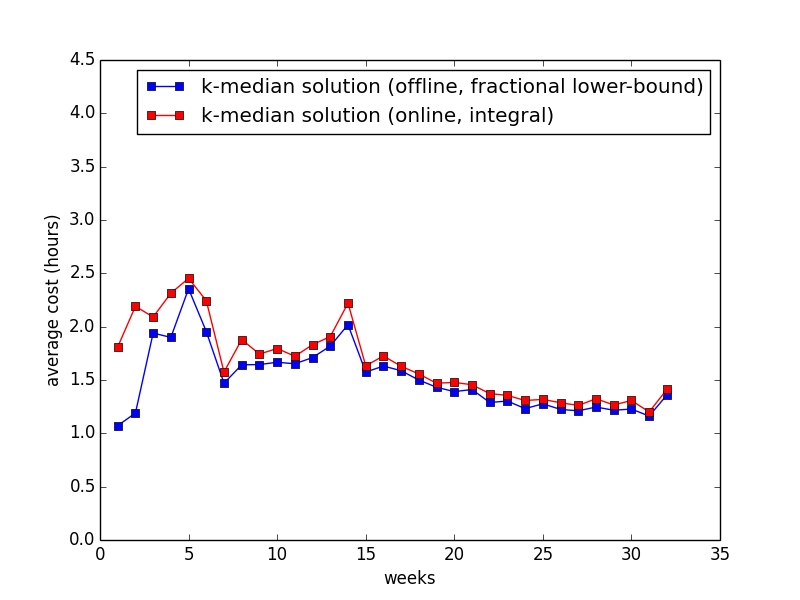
\includegraphics[width=0.30\textwidth]{figs/plot_kmed_CAP100.png}
    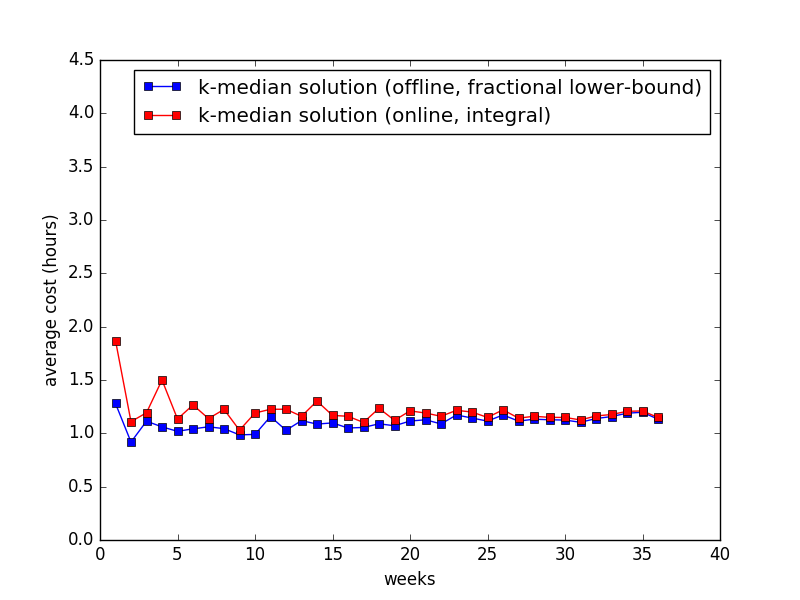
\includegraphics[width=0.30\textwidth]{figs/plot_kmed_CAP100_SL.png}
    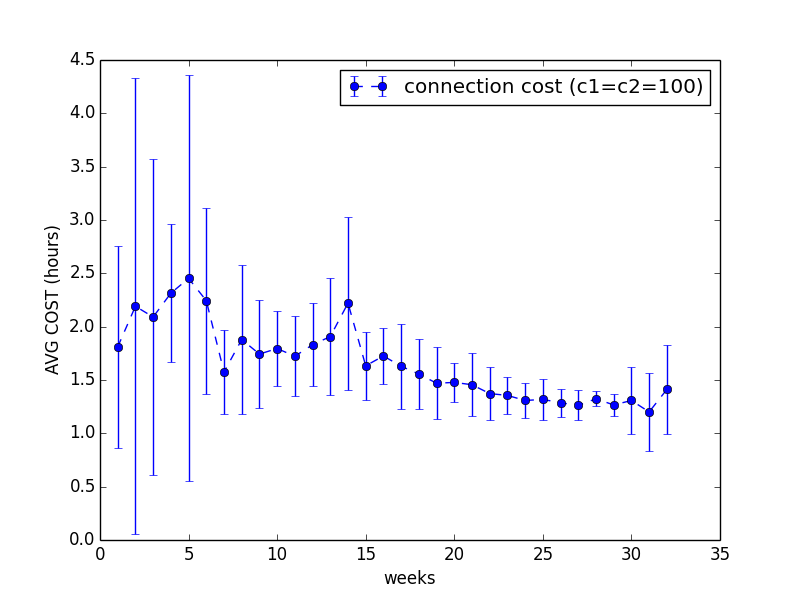
\includegraphics[width=0.3\textwidth]{figs/plot_online_cap100.png}
    \caption{Comparing the static and incremental strategies for
$s=1$, $w=2$, $k=5, k' = 2$, $cap_1 = cap_2 = 100$ for
(a) Liberia, and (b) Sierra Leone.
The variance in the solution costs over multiple iterations is shown in (c).}
\label{fig:online1}
\end{figure}

\begin{figure}[h]
  \centering % left bottom right top
    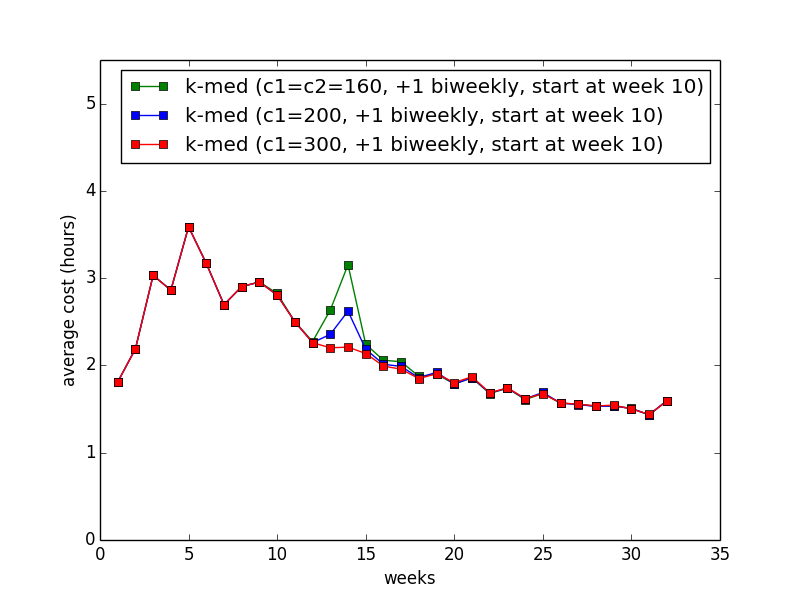
\includegraphics[width=0.45\textwidth]{figs/plot_kmed_c1.png}
    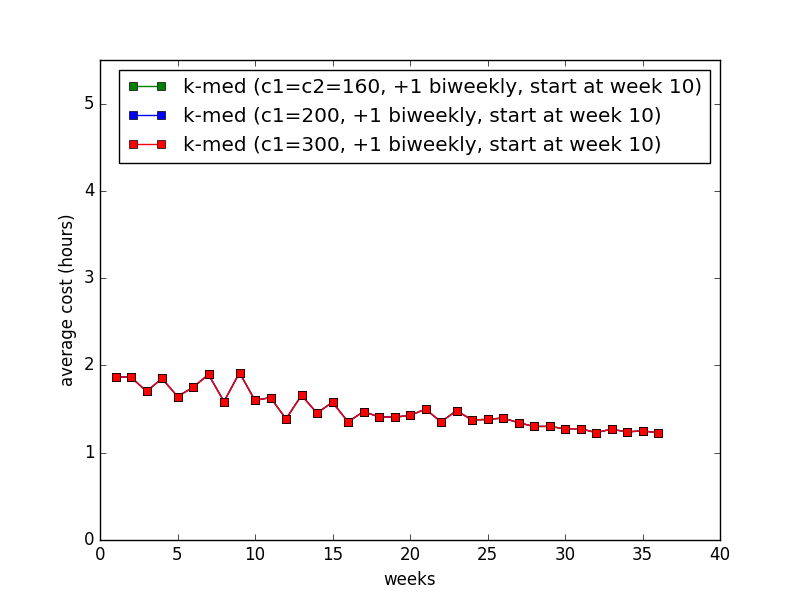
\includegraphics[width=0.45\textwidth]{figs/plot_kmed_c1c2_SL.png}
    \caption{Effect of the initial capacity $cap_1$ on the incremental solution, with
parameters $s = 10, w = 2, k' = 1, cap_2 = 160$, for (a) Liberia, and (b) Sierra Leone.}
\label{fig:online2}
\end{figure}

\begin{figure}[h]
  \centering % left bottom right top
    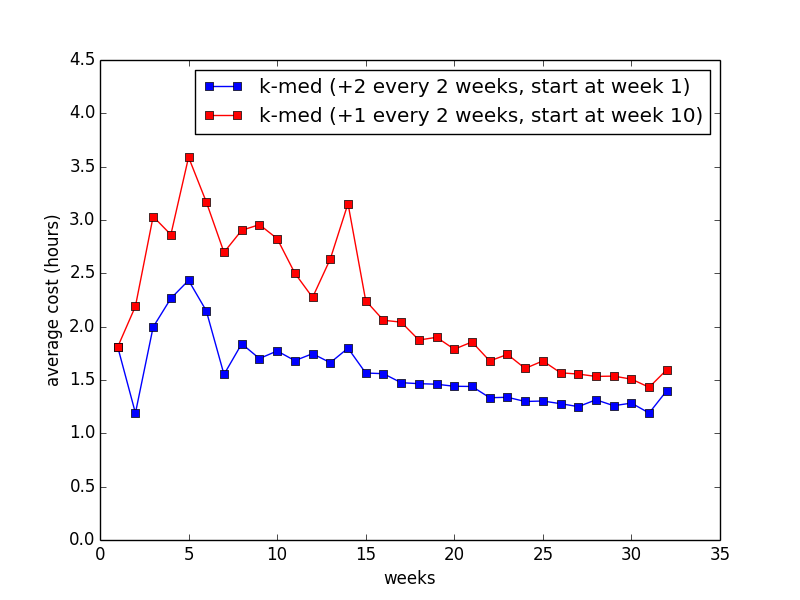
\includegraphics[width=0.45\textwidth]{figs/plot_kmed_CAP160_s1_s10.png}
    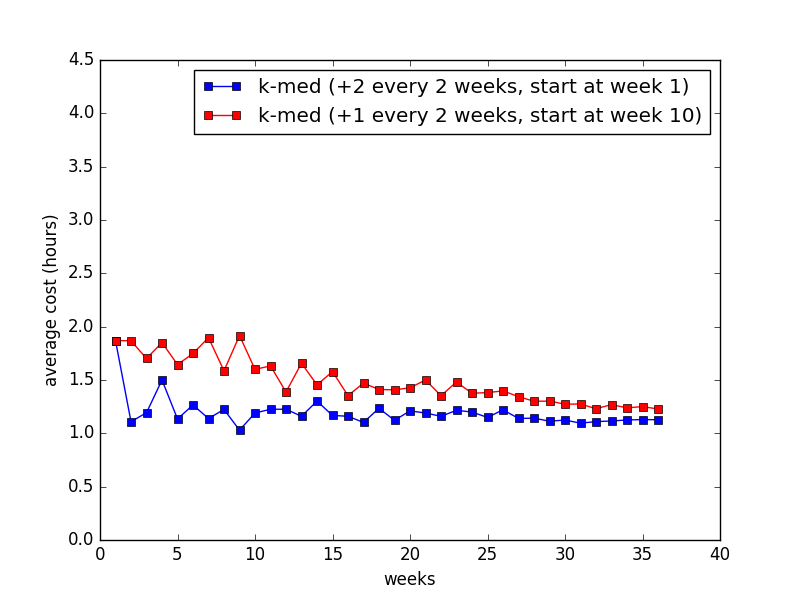
\includegraphics[width=0.45\textwidth]{figs/plot_kmed_CAP160_s1_s10_SL.png}
    \caption{Two different opening policies, with kernel size = $5$, for
(a) Liberia and (b) Sierra Leone.}
\label{fig:online3}
\end{figure}




% Place tables after the first paragraph in which they are cited.



%PLOS does not support heading levels beyond the 3rd (no 4th level headings).


\section*{Discussion}
%%
The standard $k$-median problem attempts to open a facility set which optimizes global welfare by minimizing the average travel time per person, or equivalently, the total travel time of all people. One concern is that if a small percentage of the population were located in difficult-to-reach areas, it might skew the set of facilities opened in a way that significantly lowers the global quality of the solution. This effect can be very dramatic in the $k$-supplier problem, where one bad client can single-handedly force a hospital to be opened in an otherwise unhelpful location. 

Consider the following simple example. Suppose the population exists in a single, tight cluster, except for one client who lives 30km away. Also suppose we may only open one facility.  However, the optimal solution to $k$-supplier will prefer a location halfway between the tight population cluster and the single client, such that all clients have to travel 15km. This is the most fair solution in the $k$-supplier sense, but it would be much more beneficial globally to open the facility within the tight cluster, so that most clients are extremely close, and only one client must travel 30km. 

If we are allowed to ignore a small number of people, can the average connection cost of the remaining population be significantly improved? To explore this question we develop two modified formulations of the $k$-median problem. These formulations address the following two questions. First, how well does the $k$-median solution do at minimizing the travel time of some fraction of the population of the population? Secondly, how well does the $k$-median solution do at maximizing the amount of people which obtain a specific travel time? Next, we will consider these formulations.

\subsubsection*{Minimizing cost of closest clients}
Given a cutoff distance $D$ and fraction $\epsilon$, we want to minimize the average cost of the closest $(1-\epsilon)n$ clients subject to the constraint that those clients are all within distance $D$ of an open facility. This is explicitly captured by the following program.

  \begin{alignat}{2}
   \text{LP1}: \text{min }   &  \sum_{i \in H, j \in P: w_{ij} \leq D} p_j d_{ij} x_{ij} \nonumber \\
    \text{s.t.} & \sum_{i \in H: w_{ij} \leq D} x_{ij} \leq 1    &\ & \forall j \in P \\
                             &  x_{ij} \leq y_i      & & \forall i \in H, j \in P: w_{ij} \leq D \\
                             & \sum_{i \in H} y_i \leq k\\                                                          %& \sum_{j \in P} p_j\left(1 - \sum_{i \in H: w_{ij} \leq D} x_{ij} \right) \leq  \epsilon \left( \sum_{j \in P}p_j \right) \\
& \sum_{j \in P} \sum_{i \in H: w_{ij} \leq D} p_j x_{ij} \geq  (1-\epsilon) \left( \sum_{j \in P}p_j \right) \\
&x_{ij}, y_i \in[0,1] &\qquad & \forall i\in H, j\in P
  \end{alignat}


We observe in Figure \ref{fig:kmed_vs_LP1} that our integral solutions to LP1 only marginally improve the travel time of the top $(1-\epsilon)n$ clients over that of the ordinary $k$-median solution. Since solving the LP1 formulation in integer form is NP-hard, we cannot tell for sure if there exist solutions which perform closer to the theoretical minimum given by the fractional LP solution. However, if our solutions are close to optimal, these results indicate that on real datasets, the ordinary $k$-median solution is already quite good with respect to the LP1 optimization criteria. It is not necessary to choose some parameters $D$ and $\epsilon$ and find a solution which specifically satisfies these. As long as $k$ is large enough, the ordinary $k$-median solution already performs quite well.

\subsubsection{Maximizing number of close clients}

%For $i\in H$ and $j\in P$, let $x_{ij}$ be an indicator for population node $j$ being assigned to a hospital at $i$, and let $w_{ij}$ be the cost of such an assignment. Let $y_i$ be an indicator for a hospital being opened at location $i\in H$. Let $k$ denote the number of hospitals, and $D$ denote the {\emph ideal} maximum cost for any client. 

In this formulation, we suppose we have fixed some acceptable travel cost $D$, and wish to maximize the number of clients which have a hospital within that distance. 




\begin{alignat}{2}
\text{LP2: max}  &\sum_{j\in P}\sum_{i\in H} x_{ij}p_j  && \nonumber\\
\label{eqn:violationsA1}
\text{s.t. } &x_{ij} \leq y_i &\qquad & \forall i\in H, j\in P\\
\label{eqn:violationsA2}
& x_{ij} = 0 &\qquad & \forall i\in H, j\in P \mbox{ with }d_{ij}>D\\
\label{eqn:violationsA3}
& \sum_{i\in H} x_{ij} \le 1  &\qquad & \forall j\in P\\
\label{eqn:violationsA4}
&\sum_i y_i \leq k\\
\label{eqn:violationsA5}
&x_{ij}, y_i \in[0,1] &\qquad & \forall i\in H, j\in P
\end{alignat}

We solve this formulation for $D$ varying from 2 to 7 hours, using $k=16$. We then take the solution to ordinary $k$-medain for $k=16$, and measure how many clients lie within distance $D$ for each value. The values are compared in Figure \ref{fig:LP2_AB}. 

\begin{figure}[h]
  \centering % left bottom right top
    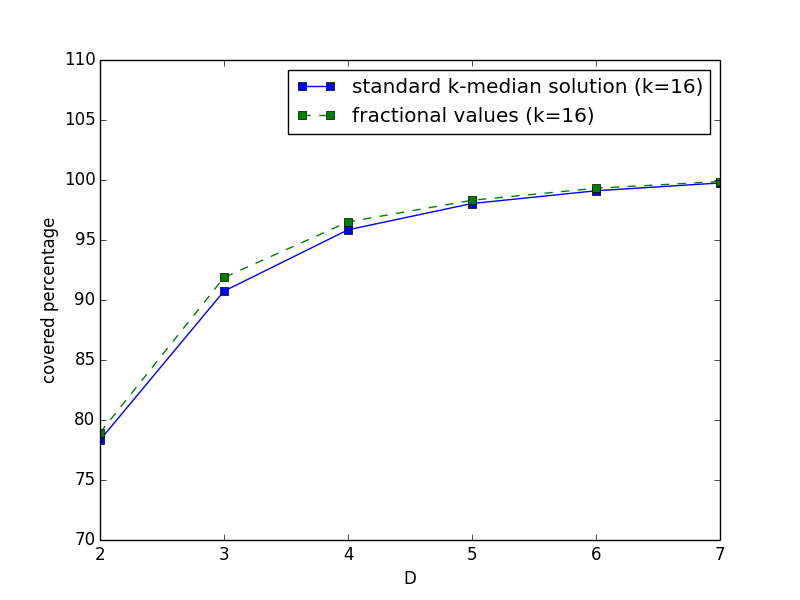
\includegraphics[width=0.4\textwidth]{figs/plotA16_min_violation.png}
	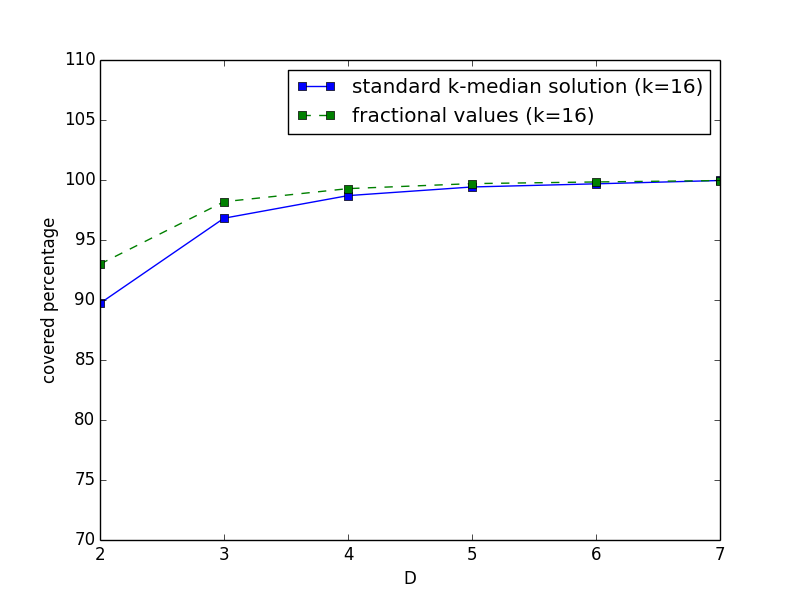
\includegraphics[width=0.4\textwidth]{figs/plotB16_min_violation.png}
\caption{Our results of solving LP2 for Dataset A (left), and B (right). (Liberia)} 
	\label{fig:LP2_AB}
\end{figure}

Figure \ref{fig:LP2_AB} shows that the $k$-median solution comes quite close to the fractional solution to LP2, which upper bounds the optimal integral solution to LP2. These results again suggest that the $k$-median solution is already quite robust, in that it already does a good job maximizing the number of clients within distance $D$, for many values of $D$ simultaneously. 

Our conclusion in this subsection is that it is only marginally beneficial to exclude any of the population as outliers. The ordinary $k$-median problem already yields a good quality solution. 




\section*{Conclusion}
%%\input{conclusion}

\section*{Supporting information}
%\subsection{Incremental facility location}
%\label{sec:incremental}

\red{details of static version here}




%\section*{Acknowledgments}


\nolinenumbers






\clearpage
\bibliographystyle{plain}
\bibliography{FacLoc,msmsort,ref}

\end{document}
